% ------------------------------------------------------------------------
% ------------------------------------------------------------------------
% Modelo UFSC para Trabalhos Academicos (tese de doutorado, dissertação de
% mestrado) utilizando a classe abntex2
%
% Autor: Alisson Lopes Furlani
% 	Modificações:
%	- 27/08/2019: Alisson L. Furlani, add pacote 'glossaries' para listas
%   - 06/11/2019: Luiz-Rafael Santos, modifica para Trabalho de Conclusão de Curso
% ------------------------------------------------------------------------
% ------------------------------------------------------------------------

\documentclass[
	% -- opções da classe memoir --
	12pt,				% tamanho da fonte
	%openright,			% capítulos começam em pág ímpar (insere página vazia caso preciso)
	oneside,			% para impressão no anverso. Oposto a twoside
	a4paper,			% tamanho do papel. 
	% -- opções da classe abntex2 --
	chapter=TITLE,		% títulos de capítulos convertidos em letras maiúsculas
	section=TITLE,		% títulos de seções convertidos em letras maiúsculas
	%subsection=TITLE,	% títulos de subseções convertidos em letras maiúsculas
	%subsubsection=TITLE,% títulos de subsubseções convertidos em letras maiúsculas
	% -- opções do pacote babel --
	english,			% idioma adicional para hifenização
	%french,				% idioma adicional para hifenização
	%spanish,			% idioma adicional para hifenização
	brazil				% o último idioma é o principal do documento
	]{abntex2}

\usepackage{setup/ufscthesisA4-alf}
\usepackage{sansmathfonts}
\usepackage[T1]{fontenc}
\renewcommand*\familydefault{\sfdefault} %% Only if the base font of the document is to be sans serif
\usepackage[version=4]{mhchem}
\DeclareUnicodeCharacter{0301}{\'{e}}
\usepackage[dvipsnames]{xcolor}
\usepackage{tikz}
\usetikzlibrary{backgrounds}
\usetikzlibrary{arrows,shapes}
\usetikzlibrary{tikzmark}
\usetikzlibrary{calc}

\usepackage{amsmath}
\usepackage{amsthm}
\usepackage{amssymb}
\usepackage{mathtools, nccmath}
\usepackage{wrapfig}
\usepackage{comment}

% To generate dummy text
\usepackage{blindtext}
\usepackage[version=4]{mhchem}
% for tikz
\usepackage{tikz}
%\usetikzlibrary{trees}
\usetikzlibrary{arrows,shapes,positioning,shadows,trees,mindmap}
% \usepackage{forest}
\usepackage[edges]{forest}
\usetikzlibrary{arrows.meta}
\colorlet{linecol}{black!75}
\usepackage{xkcdcolors} % xkcd colors


% for colorful equation
\usepackage{tikz}
\usetikzlibrary{backgrounds}
\usetikzlibrary{arrows,shapes}
\usepackage{tcolorbox}
% for custom commands
\usepackage{xspace}

% table alignment
\usepackage{array}
\usepackage{ragged2e}
\usetikzlibrary{tikzmark}
\usetikzlibrary{calc}
% Commands for Highlighting text -- non tikz method
\newcommand{\highlight}[2]{\colorbox{#1!17}{$\displaystyle #2$}}
%\newcommand{\highlight}[2]{\colorbox{#1!17}{$#2$}}
\newcommand{\highlightdark}[2]{\colorbox{#1!47}{$\displaystyle #2$}}

% my custom colors for shading
\colorlet{mhpurple}{Plum!80}


% Commands for Highlighting text -- non tikz method
% ---

% Commands for Highlighting text -- non tikz method
\renewcommand{\highlight}[2]{\colorbox{#1!17}{#2}}
\renewcommand{\highlightdark}[2]{\colorbox{#1!47}{#2}}

% Some math definitions
\newcommand{\lap}{\mathrm{Lap}}
\newcommand{\pr}{\mathrm{Pr}}

\newcommand{\Tset}{\mathcal{T}}
\newcommand{\Dset}{\mathcal{D}}
\newcommand{\Rbound}{\widetilde{\mathcal{R}}}
% Filtering and Mapping Bibliographies
% ---
% Pacotes de citações
% ---
\usepackage{csquotes}
% \usepackage[backend = biber, style = abnt]{biblatex}
% FIXME Se desejar estilo numérico de citações,  comente a linha acima e descomente a linha a seguir.
% \usepackage[backend = bibtex, style = numeric-comp]{biblatex}
\usepackage[style=numeric-comp, autocite = superscript, doi=true, sorting=none, url=false, maxcitenames=3, maxbibnames=100, block=none, backref=true]{biblatex}

\setlength\bibitemsep{\baselineskip}
\DeclareFieldFormat{url}{Disponível~em:\addspace\url{#1}}
\NewBibliographyString{sineloco}
\NewBibliographyString{sinenomine}
\DefineBibliographyStrings{brazil}{%
	sineloco     = {\mkbibemph{S\adddot l\adddot}},
	sinenomine   = {\mkbibemph{s\adddot n\adddot}},
	andothers    = {\mkbibemph{et\addabbrvspace al\adddot}},
	in			 = {\mkbibemph{In:}}
}

%\usepackage{sansmathfonts}
%\usepackage[T1]{fontenc}
%\renewcommand*\familydefault{\sfdefault}
\addbibresource{aftertext/references.bib} % Seus arquivos de referências
\usepackage{xfrac,bigints}
% ---
\DeclareSourcemap{
	\maps[datatype=bibtex]{
		% remove fields that are always useless
		\map{
			\step[fieldset=abstract, null]
			\step[fieldset=pagetotal, null]
		}
		% remove URLs for types that are primarily printed
%		\map{
%			\pernottype{software}
%			\pernottype{online}
%			\pernottype{report}
%			\pernottype{techreport}
%			\pernottype{standard}
%			\pernottype{manual}
%			\pernottype{misc}
%			\step[fieldset=url, null]
%			\step[fieldset=urldate, null]
%		}
		\map{
			\pertype{inproceedings}
			% remove mostly redundant conference information
			\step[fieldset=venue, null]
			\step[fieldset=eventdate, null]
			\step[fieldset=eventtitle, null]
			% do not show ISBN for proceedings
			\step[fieldset=isbn, null]
			% Citavi bug
			\step[fieldset=volume, null]
		}
	}
}
% ---

% ---
% Informações de dados para CAPA e FOLHA DE ROSTO
% ---
% FIXME Substituir 'Nome completo do autor' pelo seu nome.
\autor{Letícia Maria Pequeno Madureira}
% FIXME Substituir 'Título do trabalho' pelo título da trabalho.
\titulo{\textit{Balmy.jl}: Desenvolvimento de \textit{Software} para Cálculos  de Aromaticidade}
% FIXME Substituir 'Subtítulo (se houver)' pelo subtítulo da trabalho.  
% Caso não tenha substítulo, comente a linha a seguir.
\subtitulo{Implementação com ambiente gráfico}
% FIXME Substituir 'XXXXXX' pelo nome do seu
% orientador.
\orientador{Prof. Dr. Giovanni Finoto Caramori}
% FIXME Se for orientado por uma mulher, comente a linha acima e descomente a linha a seguir.
% \orientador[Orientadora]{Nome da orientadora, Dra.}
% FIXME Substituir 'XXXXXX' pelo nome do seu
% coorientador. Caso não tenha coorientador, comente a linha a seguir.
% \coorientador{Prof. XXXXXX, Dr.}
% FIXME Se for coorientado por uma mulher, comente a linha acima e descomente a linha a seguir.
% \coorientador[Coorientadora]{XXXXXX, Dra.}
% FIXME Substituir 'XXXXXX' pelo nome do Coordenador do 
% programa/curso.
% \coordenador{Prof. XXXXXX, Dr.}
% FIXME Se for coordenadora mulher, comente a linha acima e descomente a linha a seguir.
\coordenador[Coordenadora]{Nome da Coordenadora, Dra.}
% FIXME Substituir '[ano da entrega]' pelo ano (ano) em que seu trabalho foi defendido.
\ano{2022}
% FIXME Substituir '[dia] de [mês] de [ano]' pela data em que ocorreu sua defesa.
\data{15 de julho de 2022}
% FIXME Substituir '[Cidade da defesa]' pela cidade em que ocorreu sua defesa.
\local{Florianópolis}
\instituicaosigla{UFSC}
\instituicao{Universidade Federal de Santa Catarina}
% FIXME Substituir 'Dissertação/Tese' pelo tipo de trabalho (Tese, Dissertação). 
\tipotrabalho{Trabalho de Conclusão de Curso}
% FIXME Substituir '[licenciado/bacharel] em [nome do título obtido]' pela grau adequado.
\formacao{Bacharel(a) em Química}
% FIXME Substituir '[licenciado/bacharel]' pelo nivel adequado.
\nivel{Bacharel(a)}
% FIXME Substituir 'Curso de Graduação em [XXXXXXXX]' pela curso adequado.
\programa{Curso de Graduação em Química}
% FIXME Substituir 'Campus XXXXXX ou Centro de XXXXXX' pelo campus ou centro adequado.
\centro{Campus Reitor João David Ferreira Lima ou Centro de Ciências Físicas e Matemáticas}
\preambulo
{%
\imprimirtipotrabalho~do~\imprimirprograma~do~\imprimircentro~da~\imprimirinstituicao~para~a~obtenção~do~título~de~\imprimirformacao.
}
% ---

% ---
% Configurações de aparência do PDF final
% ---
% alterando o aspecto da cor azul
\definecolor{blue}{RGB}{41,5,195}
% informações do PDF
\makeatletter
\hypersetup{
     	%pagebackref=true,
		pdftitle={\@title}, 
		pdfauthor={\@author},
    	pdfsubject={\imprimirpreambulo},
	    pdfcreator={LaTeX with abnTeX2},
		pdfkeywords={ufsc, latex, abntex2}, 
		colorlinks=true,       		% false: boxed links; true: colored links
    	linkcolor=black,%blue,          	% color of internal links
    	citecolor=black,%blue,        		% color of links to bibliography
    	filecolor=black,%magenta,      		% color of file links
		urlcolor=black,%blue,
		bookmarksdepth=4
}
\makeatother
% ---

% ---
% compila a lista de abreviaturas e siglas e a lista de símbolos
% ---

% Declaração das siglas
\siglalista{HF}{Hartree-Fock}
\siglalista{RHF}{Hartree-Fock Restrito}
\siglalista{MOs}{Orbitais Moleculares}
\siglalista{AOs}{Orbitais Atômicos}
\siglalista{LCAO}{Combinação Linear de Orbitais Atômicos}
\siglalista{HOMA}{Modelo de Aromaticidade baseado em Oscilador Harmônico}
\siglalista{HMO}{Método de Hueckel}
\siglalista{HOMO}{Highest Occupied Molecular Orbital}
\siglalista{EHMO}{Método de Hueckel Estendido}

% Declaração dos simbolos

% compila a lista de abreviaturas e siglas e a lista de símbolos
\makenoidxglossaries 

% ---

% ---
% compila o indice
% ---
\makeindex
% ---

% ----
% Início do documento
% ----
\begin{document}

% Seleciona o idioma do documento (conforme pacotes do babel)
%\selectlanguage{english}
\selectlanguage{brazil}

% Retira espaço extra obsoleto entre as frases.
\frenchspacing 

% Espaçamento 1.5 entre linhas
\OnehalfSpacing

% Corrige justificação
%\sloppy

% ----------------------------------------------------------
% ELEMENTOS PRÉ-TEXTUAIS
% ----------------------------------------------------------
% \pretextual %a macro \pretextual é acionado automaticamente no início de \begin{document}
% ---
% Capa, folha de rosto, ficha bibliografica, errata, folha de apróvação
% Dedicatória, agradecimentos, epígrafe, resumos, listas
% ---
% ---
% Capa
% ---
\imprimircapa
% ---

% ---
% Folha de rosto
% (o * indica que haverá a ficha bibliográfica)
% ---
\imprimirfolhaderosto*
% ---

% ---
% Inserir a ficha bibliografica
% ---
% http://ficha.bu.ufsc.br/
\begin{fichacatalografica}
	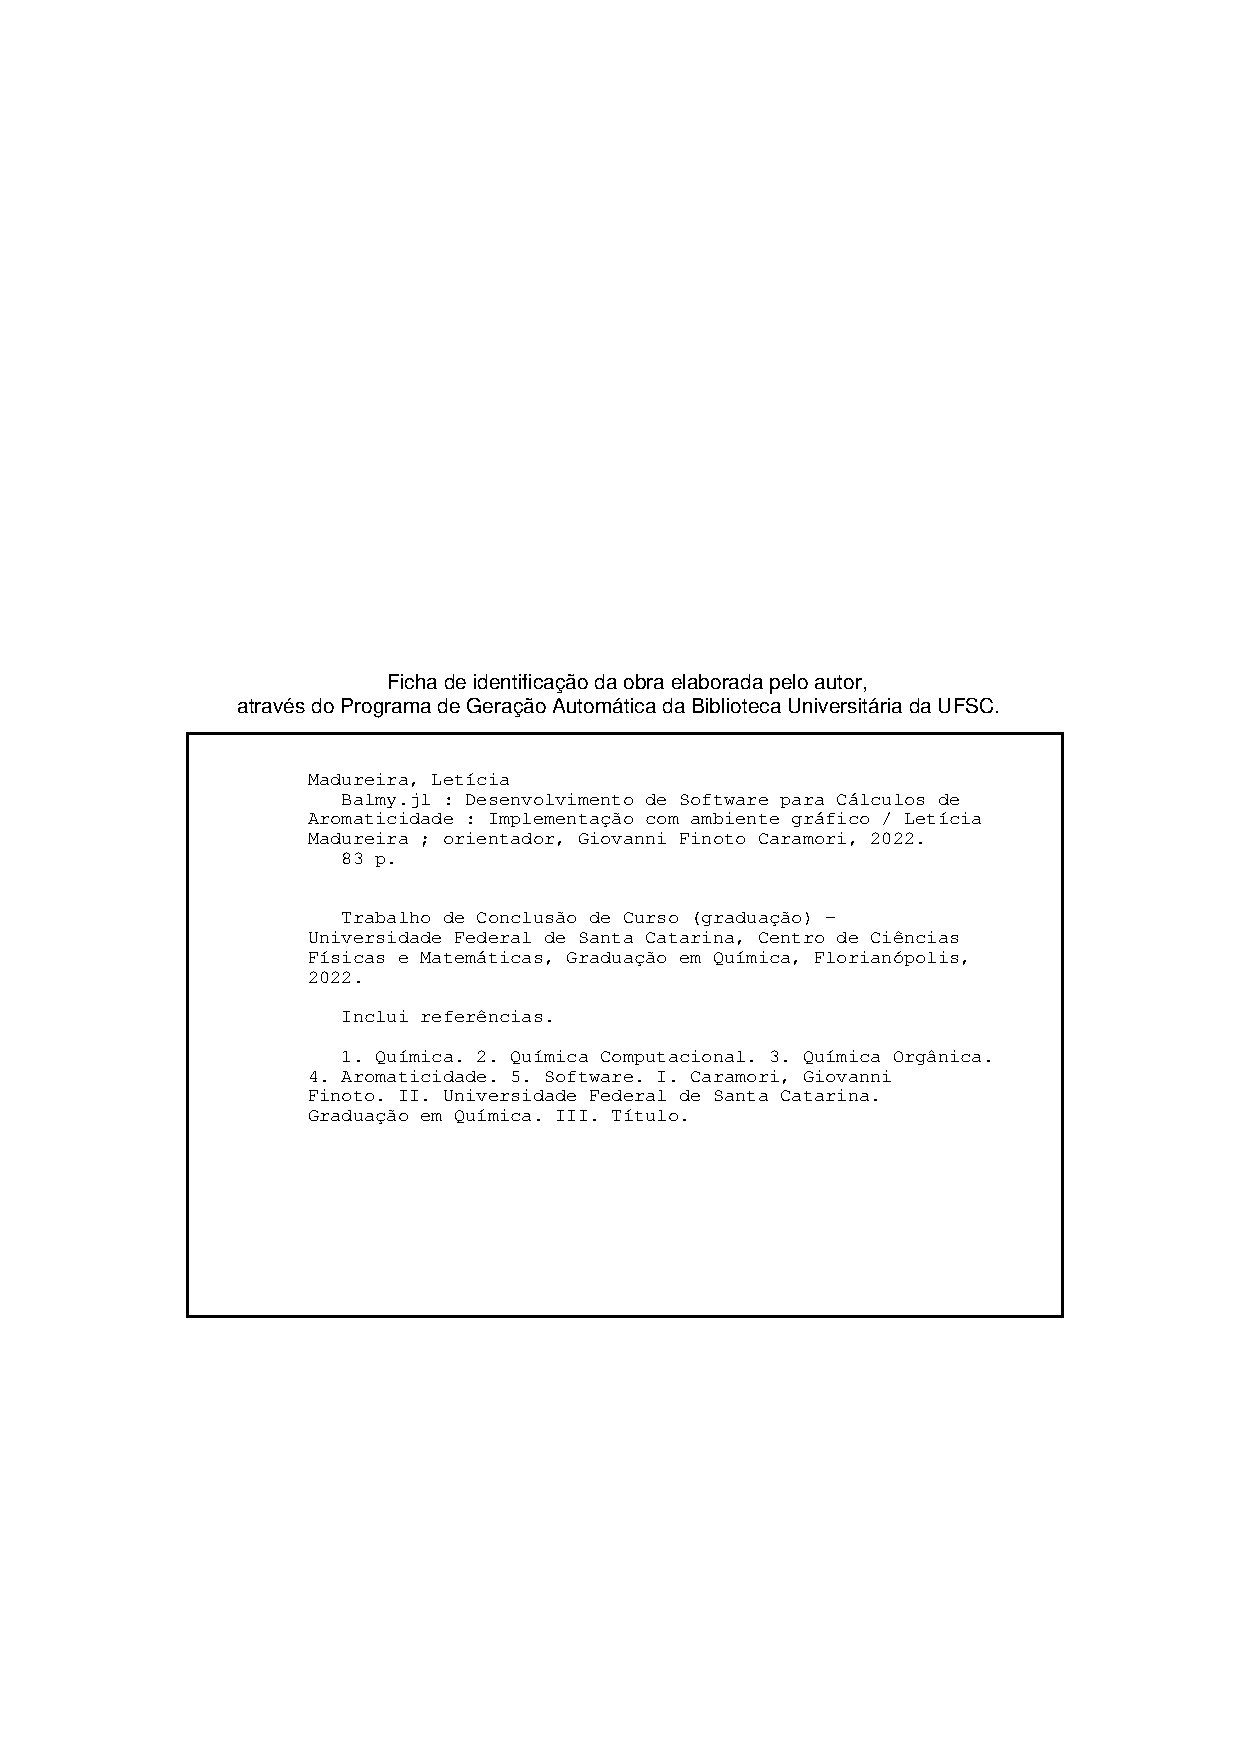
\includepdf{beforetext/Ficha_Catalografica.pdf}
\end{fichacatalografica}
% ---

% ---
% Inserir folha de aprovação
% ---
\begin{folhadeaprovacao}
	\OnehalfSpacing
	\centering
	\imprimirautor\\%
	\vspace*{10pt}		
	\textbf{\imprimirtitulo}%
	\ifnotempty{\imprimirsubtitulo}{:~\imprimirsubtitulo}\\%
	%		\vspace*{31.5pt}%3\baselineskip
	\vspace*{\baselineskip}
	%\begin{minipage}{\textwidth}
	% ~do~\imprimirprograma~do~\imprimircentro~da~\imprimirinstituicao~para~a~obtenção~do~título~de~\imprimirformacao.
	Este~\imprimirtipotrabalho~foi julgado adequado para obtenção do Título de ~\imprimirformacao~e aprovado em sua forma final pelo~\imprimirprograma. \\
		\vspace*{\baselineskip}
	\imprimirlocal, \imprimirdata. \\
	\vspace*{2\baselineskip}
	\assinatura{\OnehalfSpacing\imprimircoordenador \\ \imprimircoordenadorRotulo~do Curso}
	\vspace*{2\baselineskip}
	\textbf{Banca Examinadora:} \\
	\vspace*{\baselineskip}
	\assinatura{\OnehalfSpacing\imprimirorientador \\ \imprimirorientadorRotulo}
	%\end{minipage}%
	\vspace*{\baselineskip}
	\assinatura{Prof.(a) xxxx, Dr(a).\\
	Avaliador(a) \\
	Instituição xxxx}

	\vspace*{\baselineskip}
	\assinatura{Prof.(a) xxxx, Dr(a).\\
	Avaliador(a) \\
	Instituição xxxx}


\end{folhadeaprovacao}
% ---

% ---
% Dedicatória
% ---
\begin{dedicatoria}
	\vspace*{\fill}
	\noindent
	\begin{adjustwidth*}{}{5.5cm}     
		Este trabalho aos meus pais, meu orientador, e aos meus colegas de classe.
	\end{adjustwidth*}
\end{dedicatoria}
% ---

% ---
% Agradecimentos
% ---
\begin{agradecimentos}
	Gostaria de tecer um agradecimento primeiro à Universidade Federal de Santa Catarina e ao ensino público de qualidade (e que assim permaneça!), aos meus pais, por sempre terem me dado todo o suporte necessário para o aprendizado independentemente de qualquer entrave, e à minha irmã, por sempre ter me animado nos períodos difíceis, e aos meus 8 gatos, principalmente o Chokito, por ser o companheiro de estudos mais fiel que alguém poderia ter.

Não poderia deixar de citar todos os professores do Departamento de Química, particularmente o meu orientador Giovanni F. Caramori, que me ouviu, me ensinou e se tornou um exemplo de cientista para mim, por sua seriedade, compaixão e amor ao conhecimento. 

Seria injusto não agradecer meus colegas de laboratório, especialmente o Matheus Colaço, pelo carinho e confiança, o Felipe Schneider, pelas conversas e dicas valiosas para a construção deste projeto, e o Denner, pela amizade e descontração.

Como menção honrosa, cito a Alexandra Elbakyan, pois sem a criação do SciHub, a bibliografia do referido documento estaria vazia. Além disso, coloco aqui meu respeito a todas às mulheres na ciência e tecnologia que construíram (e que ainda hão de construir) um caminho que me possibilita estar aqui e desenvolver este trabalho. É uma grande honra fazer parte dessa história.
\end{agradecimentos}
% ---

% ---
% Epígrafe
% ---
\begin{epigrafe}
	\vspace*{\fill}
	\begin{flushright}
		\textit{``
		Classification and theory are not ends in themselves. If they generate new experimental work, new compounds, new processes, new methods - they are good;
		if they are sterile - they are bad  \\
		(Bergmann, E. D, 1971)}
	\end{flushright}
\end{epigrafe}
% ---

% ---
% RESUMOS
% ---

% resumo em português
\setlength{\absparsep}{18pt} % ajusta o espaçamento dos parágrafos do resumo
\begin{resumo}
	\SingleSpacing
	No resumo são ressaltados o objetivo da pesquisa, o método utilizado, as discussões e os resultados com destaque apenas para os pontos principais. O resumo deve ser significativo, composto de uma sequência de frases concisas, afirmativas, e não de uma enumeração de tópicos. Não deve conter citações. Deve usar o verbo na voz ativa e na terceira pessoa do singular. O texto do resumo deve ser digitado, em um único bloco, sem espaço de parágrafo. O espaçamento entre linhas é simples e o tamanho da fonte é 12. Abaixo do resumo, informar as palavras-chave (palavras ou expressões significativas retiradas do texto) ou, termos retirados de thesaurus da área. Deve conter de 150 a 500 palavras. O resumo é elaborado de acordo com a NBR 6028.
	
	\textbf{Palavras-chave}: Palavra-chave 1. Palavra-chave 2. Palavra-chave 3.
\end{resumo}

% resumo em inglês
\begin{resumo}[Abstract]
	\SingleSpacing
	\begin{otherlanguage*}{english}
		Resumo traduzido para outros idiomas, neste caso, inglês. Segue o formato do resumo feito na língua vernácula. As palavras-chave traduzidas, versão em língua estrangeira, são colocadas abaixo do texto precedidas pela expressão “Keywords”, separadas por ponto.
		
		\textbf{Keywords}: Keyword 1. Keyword 2. Keyword 3.
	\end{otherlanguage*}
\end{resumo}

%% resumo em francês 
%\begin{resumo}[Résumé]
% \begin{otherlanguage*}{french}
%    Il s'agit d'un résumé en français.
% 
%   \textbf{Mots-clés}: latex. abntex. publication de textes.
% \end{otherlanguage*}
%\end{resumo}
%
%% resumo em espanhol
%\begin{resumo}[Resumen]
% \begin{otherlanguage*}{spanish}
%   Este es el resumen en español.
%  
%   \textbf{Palabras clave}: latex. abntex. publicación de textos.
% \end{otherlanguage*}
%\end{resumo}
%% ---

{%hidelinks
	\hypersetup{hidelinks}
	% ---
	% inserir lista de ilustrações
	% ---
	\pdfbookmark[0]{\listfigurename}{lof}
	\listoffigures*
	\cleardoublepage
	% ---
	
	% ---
	% inserir lista de quadros
	% ---
	%%\pdfbookmark[0]{\listofquadrosname}{loq}
	%%\listofquadros*
	%%\cleardoublepage
	% ---
	
	% ---
	% inserir lista de tabelas
	% ---
	\pdfbookmark[0]{\listtablename}{lot}
	\listoftables*
	\cleardoublepage
	% ---
	
	% ---
	% inserir lista de abreviaturas e siglas (devem ser declarados no preambulo)
	% ---
	\imprimirlistadesiglas
	% ---
	
	% ---
	% inserir lista de símbolos (devem ser declarados no preambulo)
	% ---
	% \imprimirlistadesimbolos
	% ---
	
	% ---
	% inserir o sumario
	% ---
	\pdfbookmark[0]{\contentsname}{toc}
	\tableofcontents*
	\cleardoublepage
	
}%hidelinks
% ---
% ---

% ----------------------------------------------------------
% ELEMENTOS TEXTUAIS
% ----------------------------------------------------------
\textual

% ---
% 1 - Introdução
% ---
% ----------------------------------------------------------
\chapter{Introdução}
% ----------------------------------------------------------

A profícua evolução do processamento computacional proporcionou avanços importantes em diversas áreas do conhecimento humano, como o \textit{design} de fármacos, o planejamento sintético e a ciência de materiais, com alto potencial de aplicabilidade. Essa tendência foi observada por Gordon E. Moore \autocite{Mack2011, Shalf2020}, químico estadunidense 
cofundador da \href{https://www.intel.com/content/www/us/en/company-overview/company-overview.html}{\textit{Intel Corporation}}. A partir dele, foi cunhada uma expressão para designar o aumento bianual de 100\% no número de transistores dos chips microprocessadores, pelo mesmo custo. Isso possibilita, de maneira crescente, a implementação de ferramentas capazes de acessar - seja por meio de cálculos de estrutura eletrônica, 
simulações, ou predições - propriedades que não podem ser obtidas experimentalmente de forma direta. Isto é, uma vez que a química é uma área de difícil abstração por ser acessada na escala quântica da matéria, os computadores ocupam um lugar de destaque no estudo fenomenológico a nível macroscópico \autocite{Allouche2010, Rayan2017}.

Nesse sentido, existe uma pungente necessidade de criar novas abordagens de compreensão da química através da visualização molecular tridimensional, que por vezes faz-se mais efetiva para criar modelos mentais do que o uso de esboços bidimensionais. Importante delimitar que o termo modelagem, aqui, refere-se a um procedimento visual de interação entre a realidade e a teoria a partir de um modelo: filosófico, mecânico ou computacional \autocite{Snyder2021}, cada qual com sua respectiva aproximação. Os fenômenos físicos envolvendo os núcleos dos átomos e seus elétrons são problemas dinâmicos, de múltiplos corpos, que não têm uma solução fechada, pois sistemas quânticos possuem alta complexidade e nem sempre é possível reproduzir de forma analítica os resultados experimentais de interesse.

Esse foi exatamente o processo empenhado ao longo da história da química orgânica: estudar as relações entre as propriedades químicas e a informação estrutural retida por meio de uma compreensão preditiva embasada teoricamente. Indubitavelmente, a aromaticidade desponta nesse sentido como uma das características mais importantes das moléculas, auxiliando na interpretação de dados de reatividade, por exemplo, uma vez que compostos aromáticos apresentam uma preferência pela substituição ao invés da adição, para reter seus elétrons $\pi$ nas reações químicas. Isso foi abordado primeiramente por Roald Hoffmann \autocite{Hoffmann2014}, e desde então tornou-se uma discussão exaustiva dentro da química, sendo desenvolvidos métodos cada vez mais acurados para determinar a geometria molecular e, portanto, suas informações estruturais, como já evidenciado.

Nesse contexto, encontrar uma definição de aromaticidade que seja curta, formal e inequívoca é um desafio. Para dirimir tal dificuldade, é possível construir um conjunto de propriedades observadas em compostos que coincidem ao exibir o mesmo caráter aromático, mas de forma multidimensional. Classicamente, a aromaticidade pode ser definida pelo aumento da estabilidade termodinâmica de compostos cíclicos $\pi$-conjugados quando comparados aos seus análogos cujos elétrons são localizados.

Desse modo, é possível comprovar tal tendência avaliando a entalpia envolvida na hidrogenação ($\Delta H^\circ$) de um alceno catalisada por paládio. Tal processo é sempre exotérmico, isto é, libera uma certa quantidade de calor. Por exemplo, se analisarmos a reação de um cicloexeno (\autoref{fig:1}), o valor numérico do $\Delta H^\circ$ será -28,6 kcal/mol (\autoref{fig:2}). 

%% TODO: adicionar imagem sobre estabilização termodinâmica de compostos aromáticos

\begin{figure}[htb]
	\caption{\label{fig:1} Reação de hidrogenação de um alceno cíclico catalisada por paládio.}
	\begin{center}
		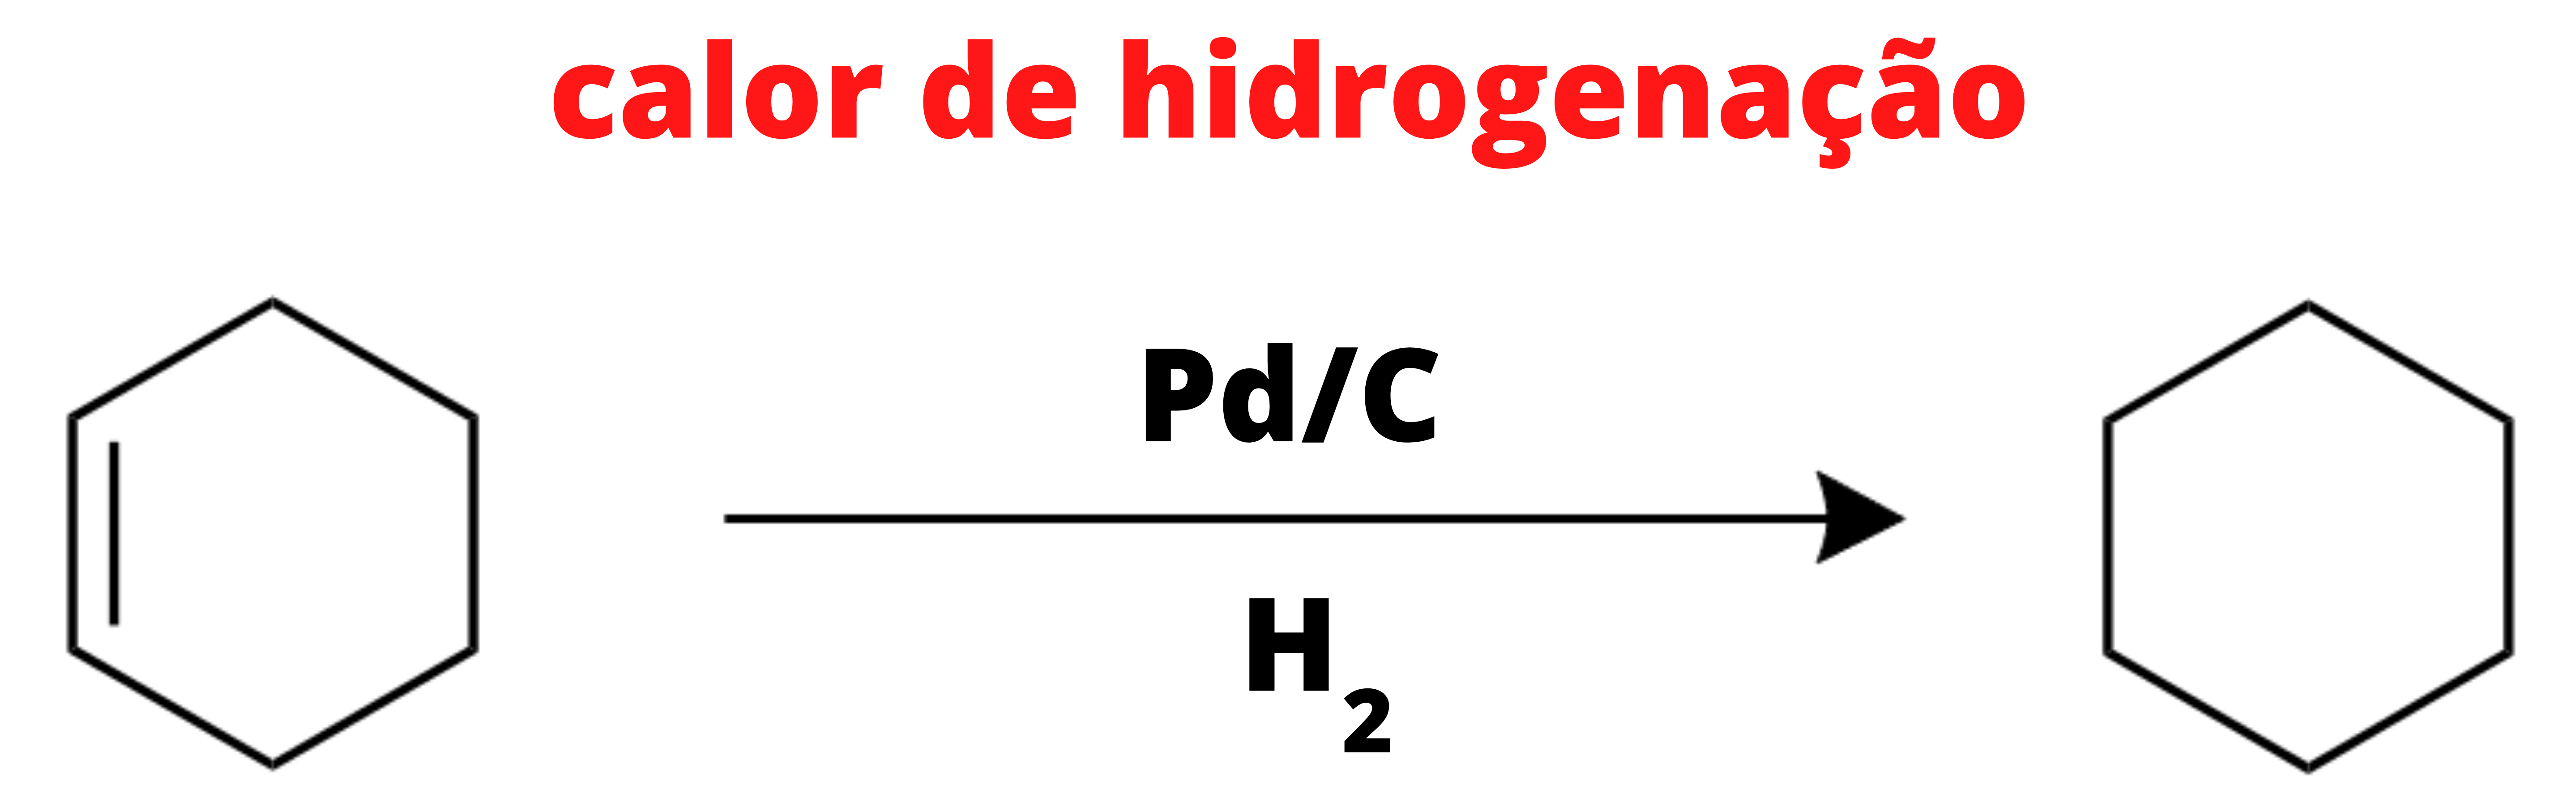
\includegraphics[width=0.5\textwidth]{images/fig1.png}
	\end{center}
	\fonte{Autor(a)}
\end{figure}

Como essa medida é aditiva, se analisarmos o caso do 1,4-cicloexadieno, que possui duas ligações duplas não conjugadas, o calor envolvido no processo será o dobro do que foi observado na situação anterior, isto é, cerca de 56 kcal/mol. No entanto, o isômero conjugado (1,3-cicloexadieno), quando hidrogenado sob as mesmas condições, libera 52,2 kcal/mol (\autoref{fig:2}). A diferença de 3,8 kcal/mol é então chamada de energia de ressonância.

Quando o anel possui três ligações duplas, como na hipótese de um cicloexatrieno, o valor numérico esperado para a entalpia de hidrogenação seria de 85,8 kcal/mol (o triplo do exemplo inicial). Porém, quando essa reação é realizada em condições normais (Pd/C, temperatura ambiente, 1 atm de H$_2$), nada acontece porque o reagente é inerte. Se a pressão for gradualmente aumentada, o cicloexatrieno permanece intacto. Finalmente, submetendo o meio a uma situação drástica (temperatura de 180-220$^\circ$C e 25-30 atm de gás hidrogênio), o reagente hipotético, enfim, gera um cicloexano. Ao medir o calor liberado, o resultado é surpreendente, uma vez que a entalpia obtida é 49,8 kcal/mol, ou seja, 36 kcal/mol abaixo do resultado que era previsto (\autoref{fig:2}). Acontece que o substrato do meio reacional em questão é o benzeno, uma estrutura totalmente conjugada e, por conseguinte, estabilizada pela sobreposição dos orbitais p \autocite{Shaabani2008, Xu2021}. Em função disso, torna-se indispensável a análise comparativa das energias associadas aos orbitais moleculares (MOs), uma vez que o caráter covalente da ligação aumenta, e a diferença de energia entre os orbitais de fronteira diminui quando comparamos as espécies aromáticas e seus análogos sem conjugação.

\begin{figure}[htb]
	\caption{\label{fig:2} Calores de hidrogenação relativos aos hidrocarbonetos cíclicos. Em vermelho, são mostradas as energias de estabilização aromática de cada um dos compostos.}
	\begin{center}
		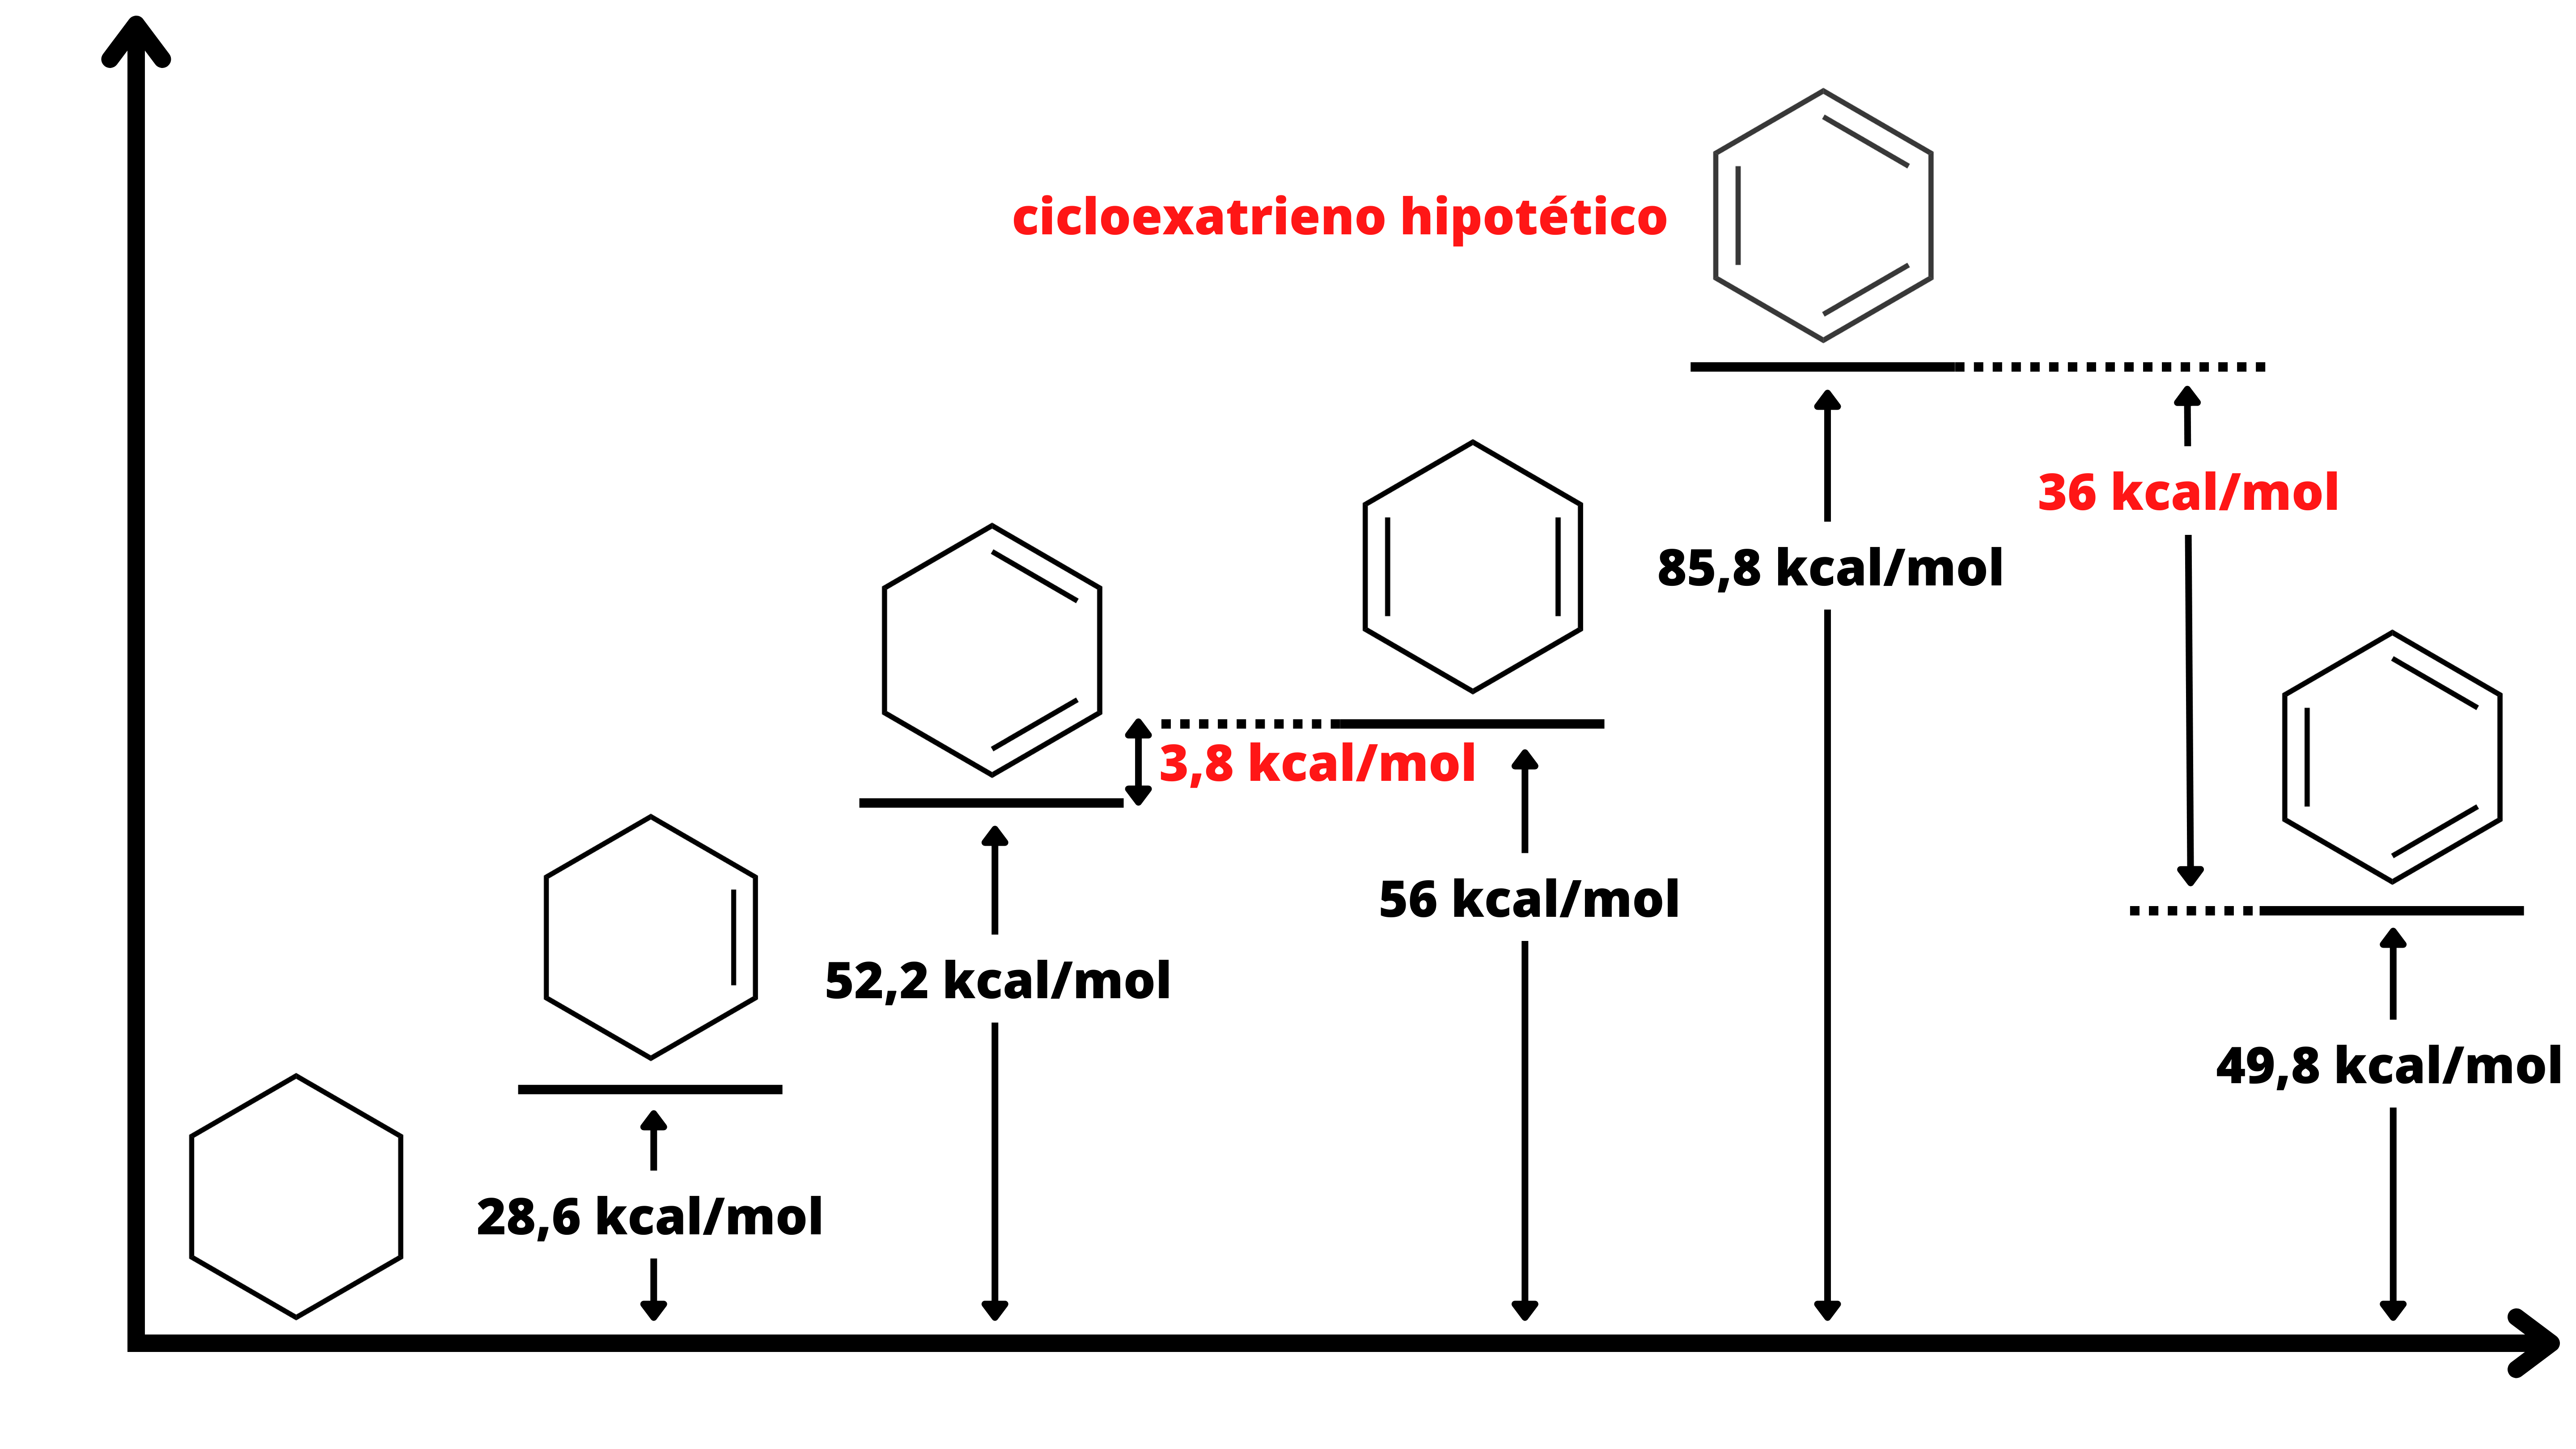
\includegraphics[width=1.0\textwidth]{images/fig2.png}
	\end{center}
	\fonte{Autor(a)}
\end{figure}

%% TODO: falar dos orbitais moleculares de fronteira na aromaticidade.

Como o conceito de aromaticidade é multidimensional\footnote{A multidimensionalidade refere-se ao fato de que o fenômeno da aromaticidade não corresponde, na maioria das vezes, aos mesmos aspectos observados.}, um problema recorrente nessas representações é que um dado critério utilizado para classificar esses compostos não pode, em geral, ser aplicado de maneira consistente. Em muitos casos, encontrar um ponto de referência apropriado é problemático. Por exemplo, os valores de energia de estabilização aromática dependem profundamente dos sistemas de referência em reações virtuais, uma vez que é praticamente impossível deduzir diferenças na aromaticidade de acordo com tendências de reatividade, a menos que sejam consideradas séries de reações estruturalmente similares, a citar, os hidrocarbonetos benzenoides \autocite{Ciesielski2009, Krygowski2014}. Nesse sentido, índices baseados na geometria molecular, tal como HOMA \autocite{Kruszewski1972}, também são relativos à escala arbitrária definida previamente.

De acordo com McWeeny, existem também muitas outras noções nos laboratórios de química e nas discussões científicas que podem ser classificadas como padrões fundamentais de entendimento (para além da aromaticidade), pois são lançados mão quase que diariamente para compreender processos químicos de maneira intuitiva. De forma mais específica, podem ser mencionados os termos: confôrmero, nucleófilo, eletrófilo, efeito de solvente, ligações de hidrogênio, acidez/basicidade de Lewis. Para analisar isso mais de perto, e de forma comparativa, foi contabilizado o número de trabalhos científicos por dia que citam alguns desses termos. Os dados mostrados na \autoref{fig:3} foram coletados do a partir de uma busca avançada no \href{https://www-periodicos-capes-gov-br.ez46.periodicos.capes.gov.br/index.php?}{\textit{Portal da Capes}}.

\begin{figure}[htb]
	\caption{\label{fig:3} Gráfico que relaciona a média de artigos científicos publicados por dia contendo cada um dos termos mostrados na legenda.}
	\begin{center}
		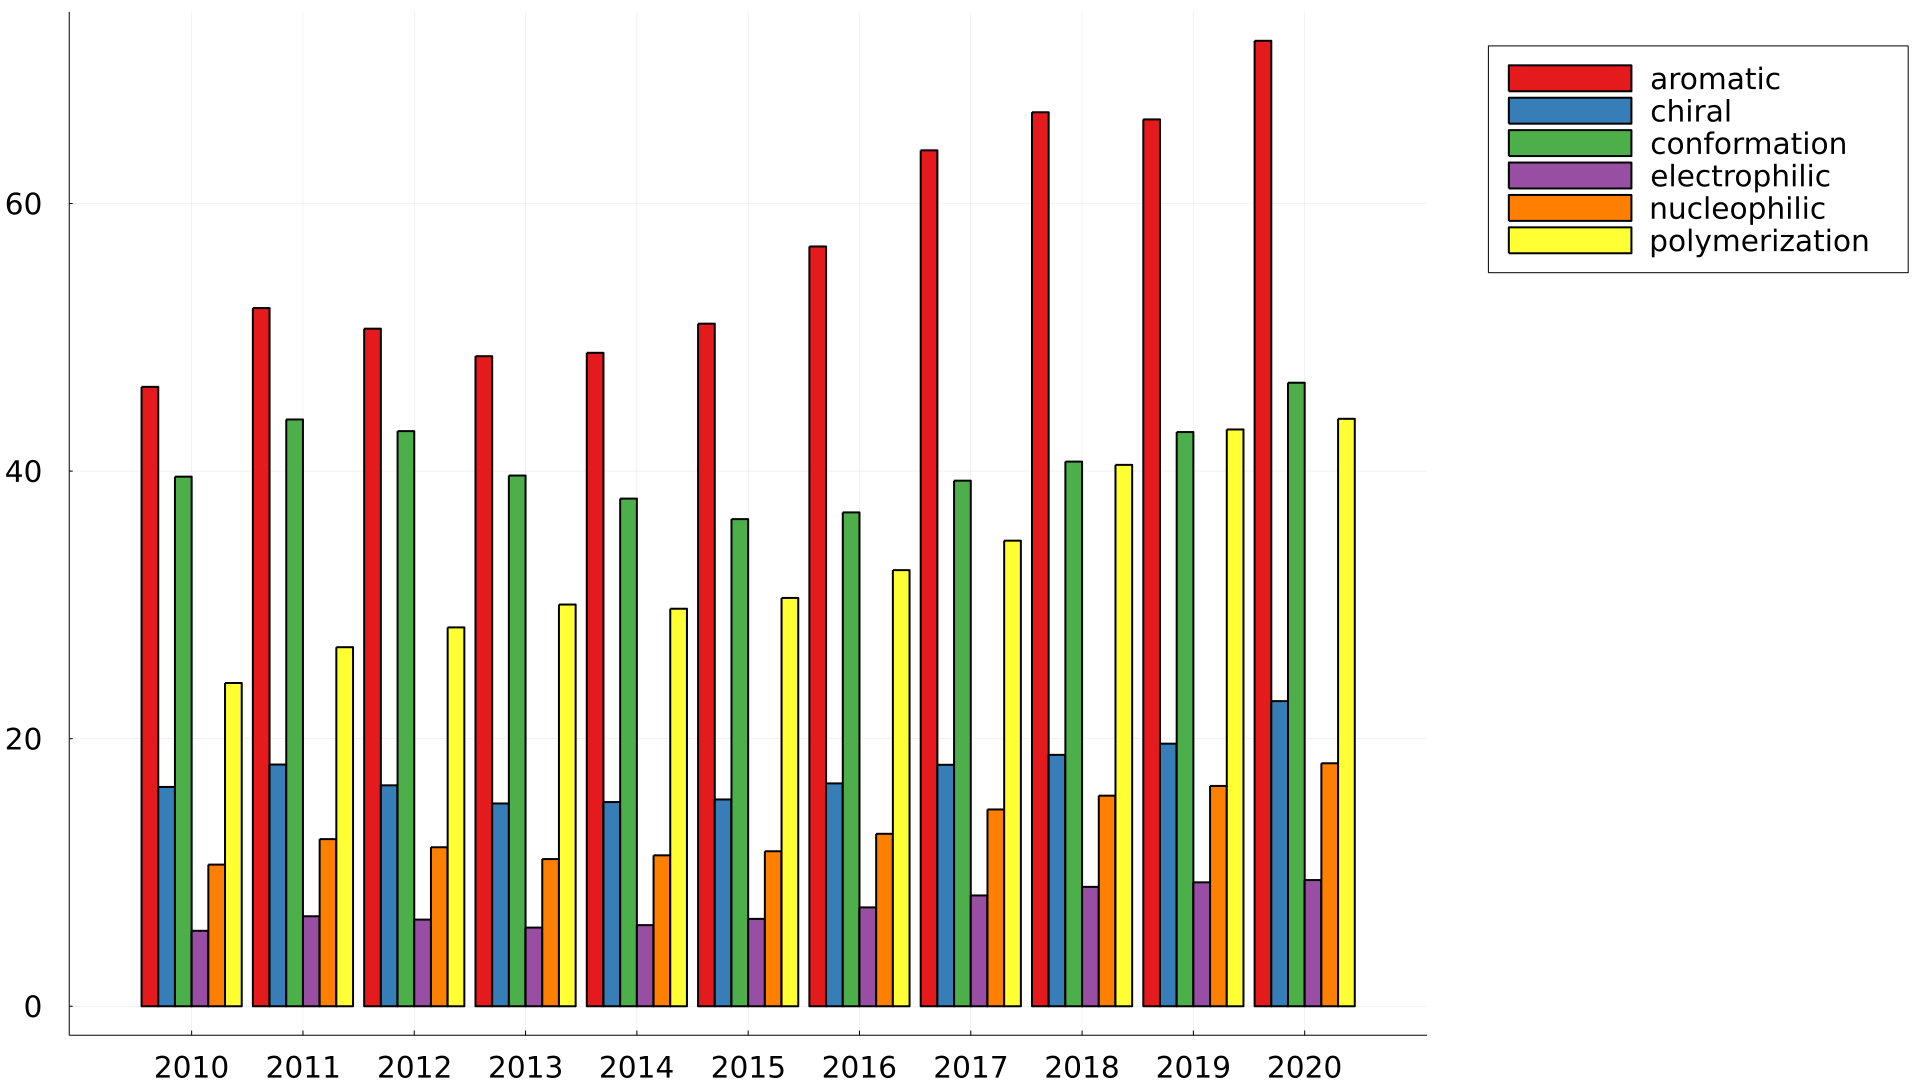
\includegraphics[width=1.0\textwidth]{images/fig3.png}
	\end{center}
	\fonte{Autor(a). Os números são do \href{https://www-periodicos-capes-gov-br.ez46.periodicos.capes.gov.br/index.php?}{\textit{Portal da Capes}}.}
\end{figure}

É possível notar, através dessa pesquisa, que o tópico da aromaticidade ocupou o topo das pesquisas durante todo o período analisado, com uma média de 60 artigos publicados por dia nos últimos anos do gráfico. 


% Ou seja, a computação gráfica auxilia na manipulação/representação direta dos objetos de estudo químico, sendo eles: átomos, moléculas (leia-se quaisquer agregados atômicos, independentemente da origem de suas interações) ou partes delas. Como esses são elementos de difícil abstração, uma vez que 

% Em tal seguimento, um dos avanços mais importantes é a aplicação da teoria de grafos à notação química e aos sistemas de busca de subestruturas e cálculos de propriedades, como a aromaticidade, que é muito sensível à geometria do sistema $\pi$, pois descreve as moléculas estabilizadas energeticamente pela deslocalização de elétrons móveis em ciclos (geometrias fechadas). Tal temática é extremamente explorada por trabalhos que vem sendo somados desde a primeira citação de Hoffmann na literatura, em 1855. Por exemplo, com uma busca sobre os termos aromático/aromaticidade no \textit{\href{https://scholar.google.com.br/scholar?hl=pt-BR&as_sdt=0\%2C5&as_ylo=2016&as_yhi=2022&q=aromatic&btnG=}{Google Scholar}} no período de 2016 a 2022, foram encontrados mais de 380 trabalhos/dia publicados, sendo a maioria destes na área de Química, uma vez que, entre os compostos carbocíclicos, destacam-se os derivados aromáticos, cuja estabilidade e reatividade dependem do caráter de deslocalização eletrônica. Para tais sistemas, é possível utilizar a equalização dos comprimentos de ligação como principal critério geométrico de análise quantitativa.


O presente trabalho pretende, fundamentado nesse conjunto de informações, relacionar as propriedades extraídas das representações moleculares a partir da computação gráfica, produzindo uma interface para manipular esses compostos de forma facilitada e didática. Uma vez que as dificuldades de compreensão por parte dos graduandos em relação aos conceitos e fenômenos originam-se na forma com que são apresentados \autocite{Cunha2018}, a ferramenta proposta poderá ser difundida para uso didático-pedagógico, podendo ser utilizada por discentes e docentes durante as aulas no sentido de demonstrar os modelos de classificação e a multidimensionalidade da aromaticidade, facilitando o entendimento.

% Assim, usuário será capaz de calcular os parâmetros geométricos de aromaticidade, um conceito explorado de forma superficial e pouco visual dentro das salas de aula. 

% ----------------------------------------------------------
\chapter{Revisão Bibliográfica}
% ----------------------------------------------------------

Historicamente, as primeiras evidências do uso da terminologia \textit{aromática(o)} remontam ao ano de 1800, mais especificamente à classificação qualitativa\footnote{Importante ressaltar que a noção de \textit{classificação qualitativa} citada pelo trabalho refere-se ao fato de, na época, não se ter conhecimento da estrutura química desses compostos.} de substâncias e óleos essenciais oriundos de produtos naturais através do odor, a exemplo da vanilina e do anetol. Nada obstante, tal ideia caiu em desuso por conduzir, mesmo na época, a associações espúrias como no caso do (-)-mentol.

Décadas depois (1825), Michael Faraday\autocite{Faraday1925, Wilson2012, Martin2015} conseguiu isolar pela primeira vez o benzeno\footnote{O nome do benzeno é derivado do ácido benzoico, descoberto no século XVI. O ácido foi assim designado por ter sido obtido pela destilação seca da goma de benjoim, uma planta nativa da Sumatra, descrita pela primeira ver por Nostradamus em 1555, depois por Aleixo Pedemontanus em 1560 e, em seguida, por Blaise de Vinagère, no ano de 1596\autocite{Nagel1990}}, um hidrocarboneto aromático com alto grau de toxicidade associado\autocite{Solomon1977}. Esse produto foi obtido por fracionamento repetido do fluido obtido durante a compressão do gás petrolífero (o acetileno, usado na iluminação das ruas de Londres, e produzido através da pirólise do óleo de baleia) fornecido através da bondade do Sr. Gordon da \href{https://portablegas.co.uk/}{\textit{Portable Gas Company}}. Ele deduziu que a fórmula molecular do composto obtido correspondia ao "bicarbureto de hidrogênio" ($C_6H_3$), baseado na massa do hidrogênio, que na época era incorreta. No entanto, ele determinou o ponto de ebulição associado ao produto final, além da sua densidade, com certa acurácia e, ao comparar seus dados com aqueles retidos do \textit{trans}-2-buteno, o qual Faraday também isolou, notou que era muito mais reativo do que o benzeno. Esse episódio representa um marco extremamente significativo para a construção da ideia de aromaticidade, uma vez que o benzeno é inegavelmente o composto mais famoso dessa classe de moléculas com propriedades derivadas da deslocalização de elétrons $\pi$\autocite{Faraday1825}. 

Poucos anos depois, em 1834, Eilhard Mitscherlich também realizou a síntese do benzeno, mas agora partindo do ácido benzoico. Esse processo ocorre sob aquecimento na presença de cal virgem ($CaO$), produzindo o benzeno como destilado do meio reacional e calcário ($CaCO_3$). Uma alternativa foi proposta por Mansfield (1845), que isolou o benzeno a partir do alcatrão de hulha sob um procedimento que \textit{a posteriori} foi adaptado à indústria. Apesar da fórmula molecular $C_6H_6$ já ser conhecida em meados do século XIX, restavam muitas dúvidas sobre os aspectos estruturais do benzeno, uma vez que essa era uma área em defasagem na época. 

A partir de 1860 os químicos estruturalistas; como Loschimidt (1861) Laderburg (1869), Claus (1866) e Dewar (1866), começaram a intencionar hipóteses sobre a estrutura do benzeno, até chegar, em 1865, na proposta de Kekulé, que se assemelha mais ao que seria a real representação estrutural do composto, fato que só foi devidamente reconhecido décadas mais tarde (1890) e comprovado em 1929\autocite{Lonsdale1929}, com a obtenção da primeira estrutura de raios-X de um derivado, o hexametilbenzeno. A base que sustenta até hoje esse modelo foi relatada inicialmente em todo o seu trabalho envolvendo os ácidos benzóico e salicílico, de ordem crucial para o avenço de diversos conceitos químicos.

Com a virada do século XIX para o XX, passou-se a ganhar entendimento da inexistência de um equilíbrio formal entre as formas isoláveis do benzeno, mas sim das estruturas canônicas de ressonância que perfazem um híbrido com elétrons móveis através de um efeito isomérico chamado mesomeria \autocite{Murrell1956, INGOLD1934, Oudar1975}. Os compostos insaturados aromáticos possuem, também, propriedades aditivas inerentes aos átomos e ligações que os constituem, como a exaltação da susceptibilidade magnética\autocite{Schleyer1996, Schleyer2001, Schleyer2014}. Segundo Pascal (1910) no artigo intitulado \textit{Magnetochemical researches}\autocite{pascal1910magnetochemical}, a mobilidade eletrônica em estruturas cujas ligações duplas são alternadas torna-as diamagnéticas, isto é, não possuem magnetização a campo zero e apresentam uma magnetização contrária quando um campo é aplicado. Por isso, os compostos aromáticos são capazes de induzir campos magnéticos significativos a ponto de interferir nas frequências de ressonância de átomos ligados ao anel aromático. Neste caso, são conhecidos os efeitos de proteção e desproteção de núcleos provocados pelas correntes de anel.

Foi então no ano de 1931, quando a fundamentação estrutural da aromaticidade se tornava mais sólida, que surgiu uma das primeiras regras de classificação de moléculas aromáticas desenvolvida por Erich Hueckel\autocite{Hckel1931}. Utilizando a teoria dos orbitais moleculares, ele elucidou muitos pontos sobre as propriedades eletrônicas de compostos orgânicos, o que o permitiu demonstrar que hidrocarbonetos cíclicos com (4$n$+2) elétrons $\pi$ (sendo $n$ um número inteiro) possuem um incremento da estabilidade energética. Hueckel\autocite{Hckel1931, Brogli1972} justificou este efeito através da distribuição eletrônica dos compostos aromáticos, uma vez que, para ele, a razão do abaixamento da energia dos compostos aromáticos devia-se à ausência de elétrons desemparelhados.

Tal abordagem tem, no entanto, suas excepcionalidades, a exemplo dos $[$10$]$anulenos, que possuem o número adequado de elétrons $\pi$, mas não as demais propriedades associadas à aromaticidade (estabilidade, reatividade, propriedades magnéticas típicas e planaridade da molécula). Essa distorção é causada por fatores topológicos e efeitos estereoeletrônicos observados nesses compostos, pois os hidrogênios internos das estruturas dos [10]anulenos afetam boa conjugação do sistema $\pi$ \autocite{Caramori2006}. 

Simultaneamente, surgiram algumas estratégias experimentais para a determinação das energias de ressonância, que justificam o aumento da estabilidade dos compostos aromáticos. Pauling (1933) \autocite{Pauling1933, Pauling1936} e Kistiakowsky (1936) calcularam a energia de ressonância do benzeno baseando-se nos calores de hidrogenação ($Delta H^{\circ}_{\textrm{hidrogenação}}$) de algumas reações selecionadas. Eles encontraram valores em torno de 36 kcal/mol, o que serviu para comparar com os parâmetros já conhecidos para alcenos não conjugados e assim aprofundar o estudo físico-químico da aromaticidade. Dessa forma, com o avanço da química quântica e dos métodos teóricos de análise dos arranjos atômicos no século XX, evoluíram também os critérios para se avaliar se os compostos podem ser classificados como (\textit{i}) \textit{aromáticos} (estabilizados por ressonância de elétrons), (\textit{ii}) \textit{não-aromáticos} (não sofrem efeito mesomérico) ou (\textit{iii}) \textit{antiaromáticos} (desestabilizados por efeitos geométricos, torcionais e estereoeletrônicos); quais sejam, de origem geométrica, magnética e energética. 

% ----------------------------------------------------------
\chapter{Objetivos}
% ----------------------------------------------------------

% ----------------------------------------------------------
\section{Objetivo Geral}
% ----------------------------------------------------------

 Desenvolver um \textit{software} de interação gráfica capaz de representar a molécula tridimensionalmente através da leitura de dados de coordenadas cartesianas atômicas e assim retornar parâmetros de aromaticidade segundo a metodologia definida pelo usuário. Poderá, portanto, ser utilizado como uma ferramenta de pós-processamento para o cálculo de propriedades eletrônicas. Além disso, também pretende-se implementar métodos semiempíricos de baixo custo computacional (Hueckel e Hueckel estendido) para auxiliar na avaliação e representação dos orbitais atômicos e moleculares.

% ----------------------------------------------------------
\section{Objetivos Específicos}
% ----------------------------------------------------------

\begin{itemize}
    %\item Realizar pré-otimizações de geometria utilizando métodos semi-empíricos e \textcolor{red}{realizando leituras de estruturas obtidas por outros métodos através de outros \textit{softwares}; complementar};
    
    \item Utilizar métodos semiempíricos para avaliar orbitais atômicos e moleculares.
    
    \item Automatizar a leitura de arquivos de saída \textit{outputs} \textit{logfiles} de cálculos de estrutura eletrônica molecular visando extrair dados geométricos para determinar critérios de aromaticidade geométricos em sistemas orgânicos, através de uma interface gráfica.

    \item Utilizar a teoria de grafos para implementar a determinação dos índices HOMA, EN, e GEO; 
    
    \item Realizar \textit{benchmark} dos resultados obtidos com estruturas já reportadas na literatura para fins de  validação e comparação do tempo de computação na metodologia aplicada.
\end{itemize}
% ---

% ---
% 2 - Capítulo 2
% ---
% ----------------------------------------------------------
\chapter{Desenvolvimento}\label{cap:desenvolvimento}
% ----------------------------------------------------------
Deve-se inserir texto entre as seções.

% ----------------------------------------------------------
\section{Exposição do tema ou matéria}
% ----------------------------------------------------------

É a parte principal e mais extensa do trabalho. Deve apresentar a fundamentação teórica, a metodologia, os resultados e a discussão. Divide-se em seções e subseções conforme a NBR 6024 \cite{NBR6024:2012}.

Quanto à sua estrutura e projeto gráfico, segue as recomendações da  para preparação de trabalhos acadêmicos, a NBR 14724, de 2011 \cite{NBR14724:2011}.

\begin{figure}[htb]
	\caption{\label{fig:Fig_1}Elementos do trabalho acadêmico.}
	\begin{center}
		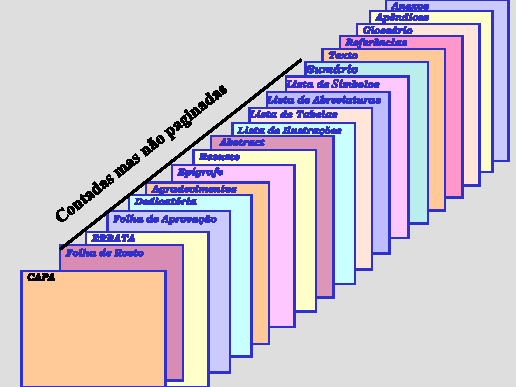
\includegraphics{images/imagem.pdf}
	\end{center}
	\fonte{Universidade Federal do Paraná (1996).}
\end{figure}

% ----------------------------------------------------------
\subsection{Formatação do texto}
% ----------------------------------------------------------

No que diz respeito à estrutura do trabalho, recomenda-se que:
\begin{alineas}
	\item o texto deve ser justificado, digitado em cor preta, podendo utilizar outras cores somente para as ilustrações;
	\item utilizar papel branco ou reciclado para impressão;
	\item  \textbf{se o trabalho for impresso}, os elementos pré-textuais devem iniciar no anverso da folha, com exceção da ficha catalográfica ou ficha de identificação da obra;
	\item \textbf{se o trabalho for impresso}, os elementos textuais e pós-textuais devem ser digitados no anverso e verso das folhas, quando o trabalho for impresso;

	\item as seções primárias devem começar sempre em páginas ímpares, quando o trabalho for impresso; e 
	\item deixar um espaço entre o título da seção/subseção e o texto e entre o texto e o título da subseção.
\end{alineas}

No \autoref{qua:Quadro_1} estão as especificações para a formatação do texto.

\begin{quadro}[htb]
	\centering
	\caption{\label{qua:Quadro_1}Formatação do texto.}	
	\begin{tabular}{|l|p{11cm}|}
		\hline
		\textbf{Formato do papel} & A4.\\ \hline
		\textbf{Impressão}        & A norma recomenda que \textbf{caso seja necessário imprimir}, deve-se utilizar a frente e o verso da página.\\ \hline
		\textbf{Margens}          & Superior: 3, Inferior: 2, Interna: 3 e Externa: 2. Usar margens espelhadas quando o  trabalho for impresso.\\ \hline
		\textbf{Paginação}        & As páginas dos elementos pré-textuais devem ser contadas, mas não numeradas. Para trabalhos digitados somente no anverso, a numeração das páginas deve constar no canto superior direito da página, a 2 cm da borda, figurando a partir da primeira folha da  parte textual. Para trabalhos digitados no anverso e no verso, a numeração deve constar no canto superior direito, no anverso, e no canto superior esquerdo no verso.\\ \hline
		\textbf{Espaçamento}      & O texto deve ser redigido com espaçamento entre linhas 1,5, excetuando-se as citações de mais de três linhas, notas de rodapé, referências, legendas das ilustrações e das tabelas, natureza (tipo do trabalho, objetivo, nome da instituição a que é submetido e área de concentração), que devem ser digitados em espaço simples, com fonte menor. As referências devem ser separadas entre si por um espaço simples em branco.\\ \hline
		\textbf{Paginação}        & A contagem inicia na folha de rosto, mas se \textbf{insere o número da página na introdução} até o final do trabalho.\\ \hline
		\textbf{Fontes sugeridas} & Arial ou Times New Roman.\\ \hline
		\textbf{Tamanho da fonte} & \textbf{Fonte tamanho 12 para o texto}, incluindo os títulos das seções e subseções. As citações com mais de três linhas, notas de rodapé, paginação, dados internacionais de catalogação, legendas e fontes das ilustrações e das tabelas devem ser de tamanho menor. Adotamos, neste \textit{template} \textbf{fonte tamanho 10}.\\ \hline
		\textbf{Nota de rodapé}   & Devem ser digitadas dentro da margem, ficando separadas por um espaço simples por entre as linhas e por filete de 5 cm a partir da margem esquerda. A partir da segunda linha, devem ser alinhadas embaixo da primeira letra da primeira palavra da primeira linha.\\ \hline
	\end{tabular}
	\fonte{\textcite{NBR14724:2011}.}
\end{quadro}

% ----------------------------------------------------------
\subsubsection{As ilustrações}
% ----------------------------------------------------------

Independentemente do tipo de ilustração (quadro, desenho, figura, fotografia, mapa, entre outros), a sua identificação aparece na parte superior, precedida da palavra designativa. 

\begin{citacao}
	Após a ilustração, na parte inferior, indicar a fonte consultada (elemento obrigatório, mesmo que seja produção do próprio autor), legenda, notas e outras informações necessárias à sua compreensão (se houver). A ilustração deve ser citada no texto e inserida o mais próximo possível do texto a que se refere. \cite[p. 11]{NBR14724:2011}.
\end{citacao}

% ----------------------------------------------------------
\subsubsection{Equações e fórmulas}
% ----------------------------------------------------------

As equações e fórmulas devem ser destacadas no texto para facilitar a leitura.  Para numerá-las, usar algarismos arábicos entre parênteses e alinhados à direita. Pode-se adotar uma entrelinha maior do que a usada no texto \cite{NBR14724:2011}. \\


\begin{figure}[htb]
    \vspace{2\baselineskip}
\begin{equation}
    \label{cor}
    R_{opt} = \frac{ \tikzmarknode{single}{ \highlight{blue}{$R_{C-C}$}} + 2 \tikzmarknode{double}{ \highlight{red}{$R_{C=C}$}}}{3} = 1.397 \textit{\AA}
\end{equation}
\begin{tikzpicture}[overlay,remember picture,>=stealth,nodes={align=left,inner ysep=1pt},<-]
    \path (single.north) ++ (-1,2em) node[anchor=south east,color=blue!67] (scalep){\textit{$R_{C-C} = 1.524$ \AA}};
    \draw [color=blue!87](single.north) |- ([xshift=-3em,color=blue]scalep.south west);
    
    \path (double.north) ++ (1,2em) node[anchor=south west, color=red!67] (scalep){\textit{$R_{C=C} = 1.334$ \AA}};
    \draw [color=red!87](double.north) |- ([xshift=3em,color=red]scalep.south east);
\end{tikzpicture}
\end{figure}

\begin{figure}[htb]
    \vspace{2\baselineskip}
\begin{equation}
    \label{correcao}
    \tikzmarknode{homa}{\highlight{blue}{HOMA}} = 1 - EN - GEO
\end{equation}
\begin{tikzpicture}[overlay,remember picture,>=stealth,nodes={align=left,inner ysep=1pt},<-]
    \path (homa.north) ++ (-2em,1.5em) node[anchor=south east,color=blue!67] (scalep){\textit{índice geométrico}};
    \draw [color=blue!87](homa.north) |- ([xshift=-3em,color=blue]scalep.south west);
\end{tikzpicture}
\end{figure}


% ----------------------------------------------------------
\subsubsubsection{Exemplo tabela}
% ----------------------------------------------------------


% ---

% ---
% 3 - Capítulo 3
% ---
% ----------------------------------------------------------
\chapter{Seção}
% ----------------------------------------------------------

Este \textit{template} contém algumas seções criadas na tentativa de facilitar seu uso. No entanto, não há um limite máximo ou mínimo de seção a ser utilizado no trabalho. Cabe a cada autor definir a quantidade que melhor atenda à sua 
necessidade.  
% ---

% ---
% 4 - Resultados
% ---
%\phantompart
% ----------------------------------------------------------
\chapter{Resultados}
% ----------------------------------------------------------

\section{Interface gráfica}\label{design}

A interface gráfica do \textit{Balmy.jl} é mostrada na \autoref{gui-pronta}. Os elementos interativos foram implementados para garantir o suporte e usabilidade do \textit{software}, sendo extremamente intuitivo e fácil de usar, pois é acessado através do navegador e, assim, pode utilizado nas salas de aula da graduação.

\begin{figure}[htb]
	\caption{\label{workflow} Fluxo de trabalho do \textit{software} produzido.}
	\begin{center}
		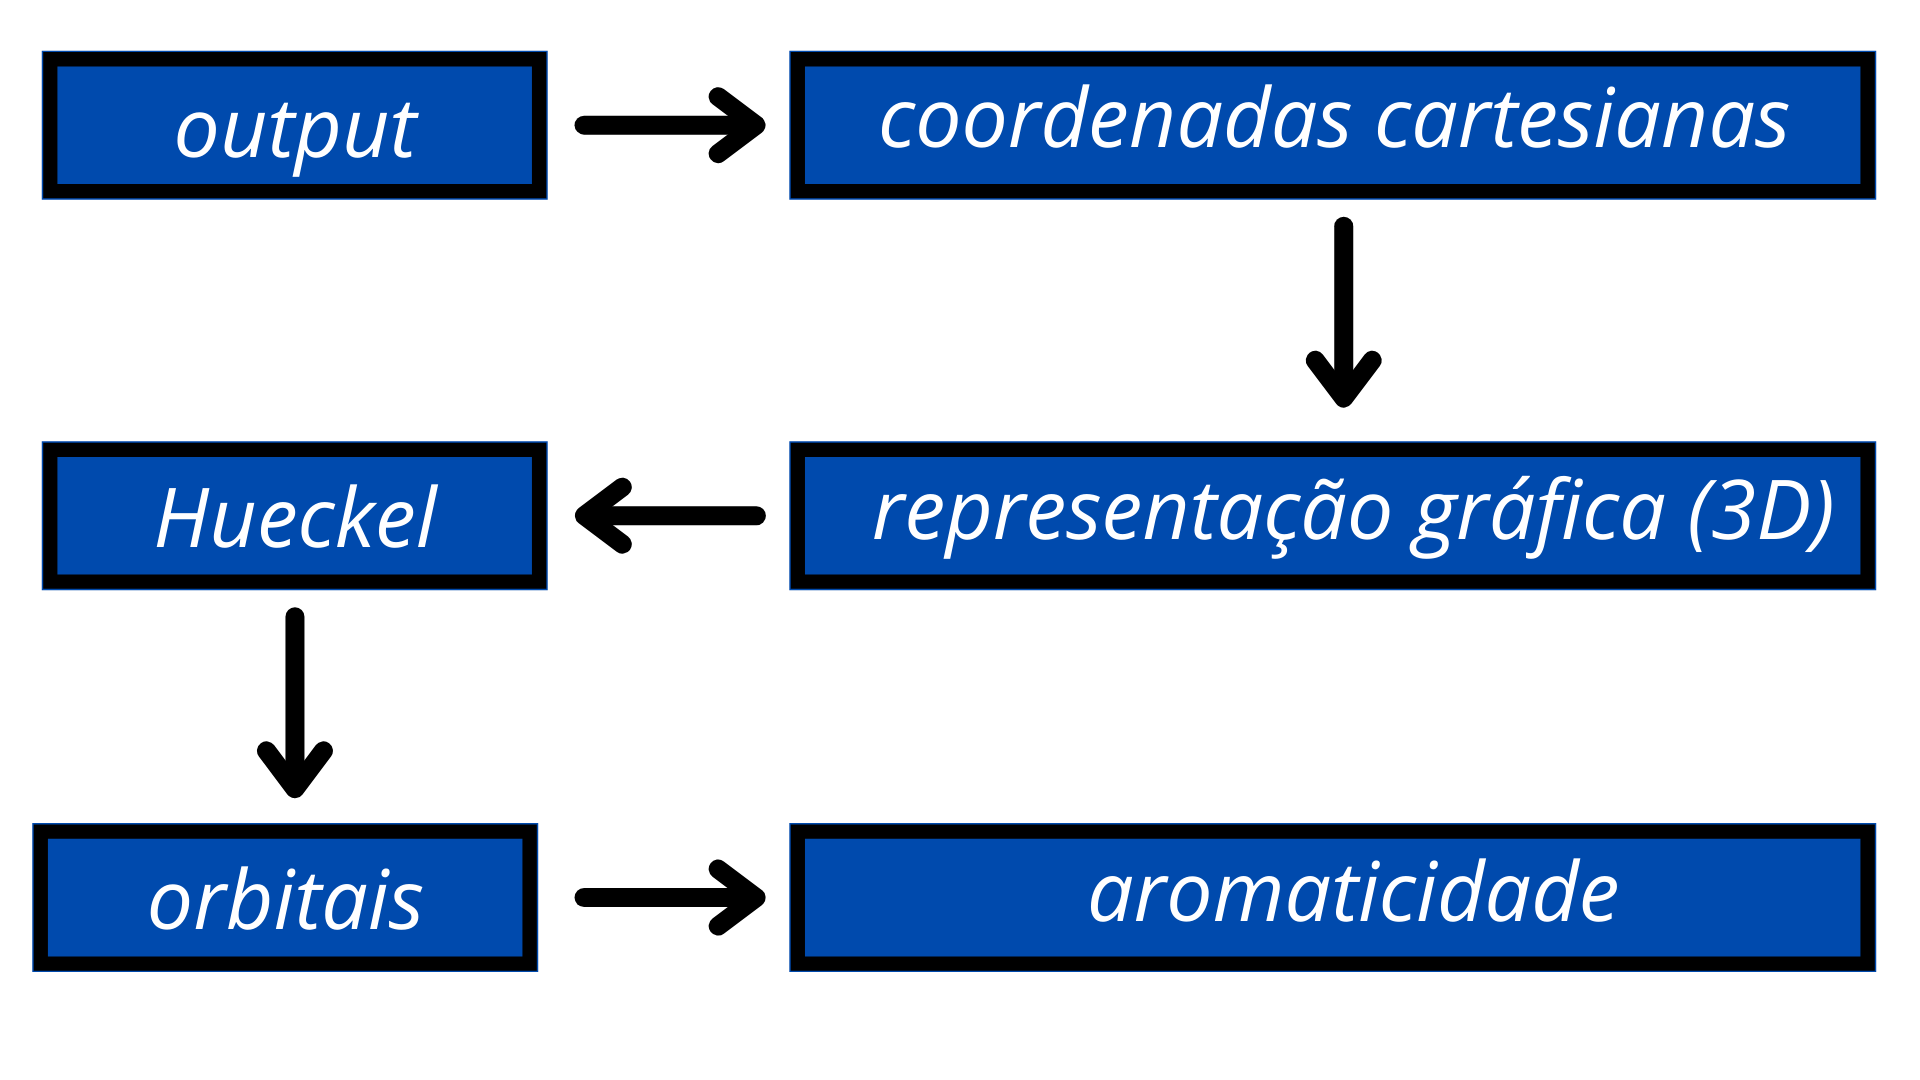
\includegraphics[width=0.6\textwidth]{images/workflow.png}
	\end{center}
	\fonte{Autor(a)}
\end{figure}

\begin{figure}[htb]
	\caption{\label{gui-pronta} Aqui é mostrada a interface gráfica produzida. Os círculos sinalizam as funções associadas às áreas da \gls{GUI}.}
	\begin{center}
		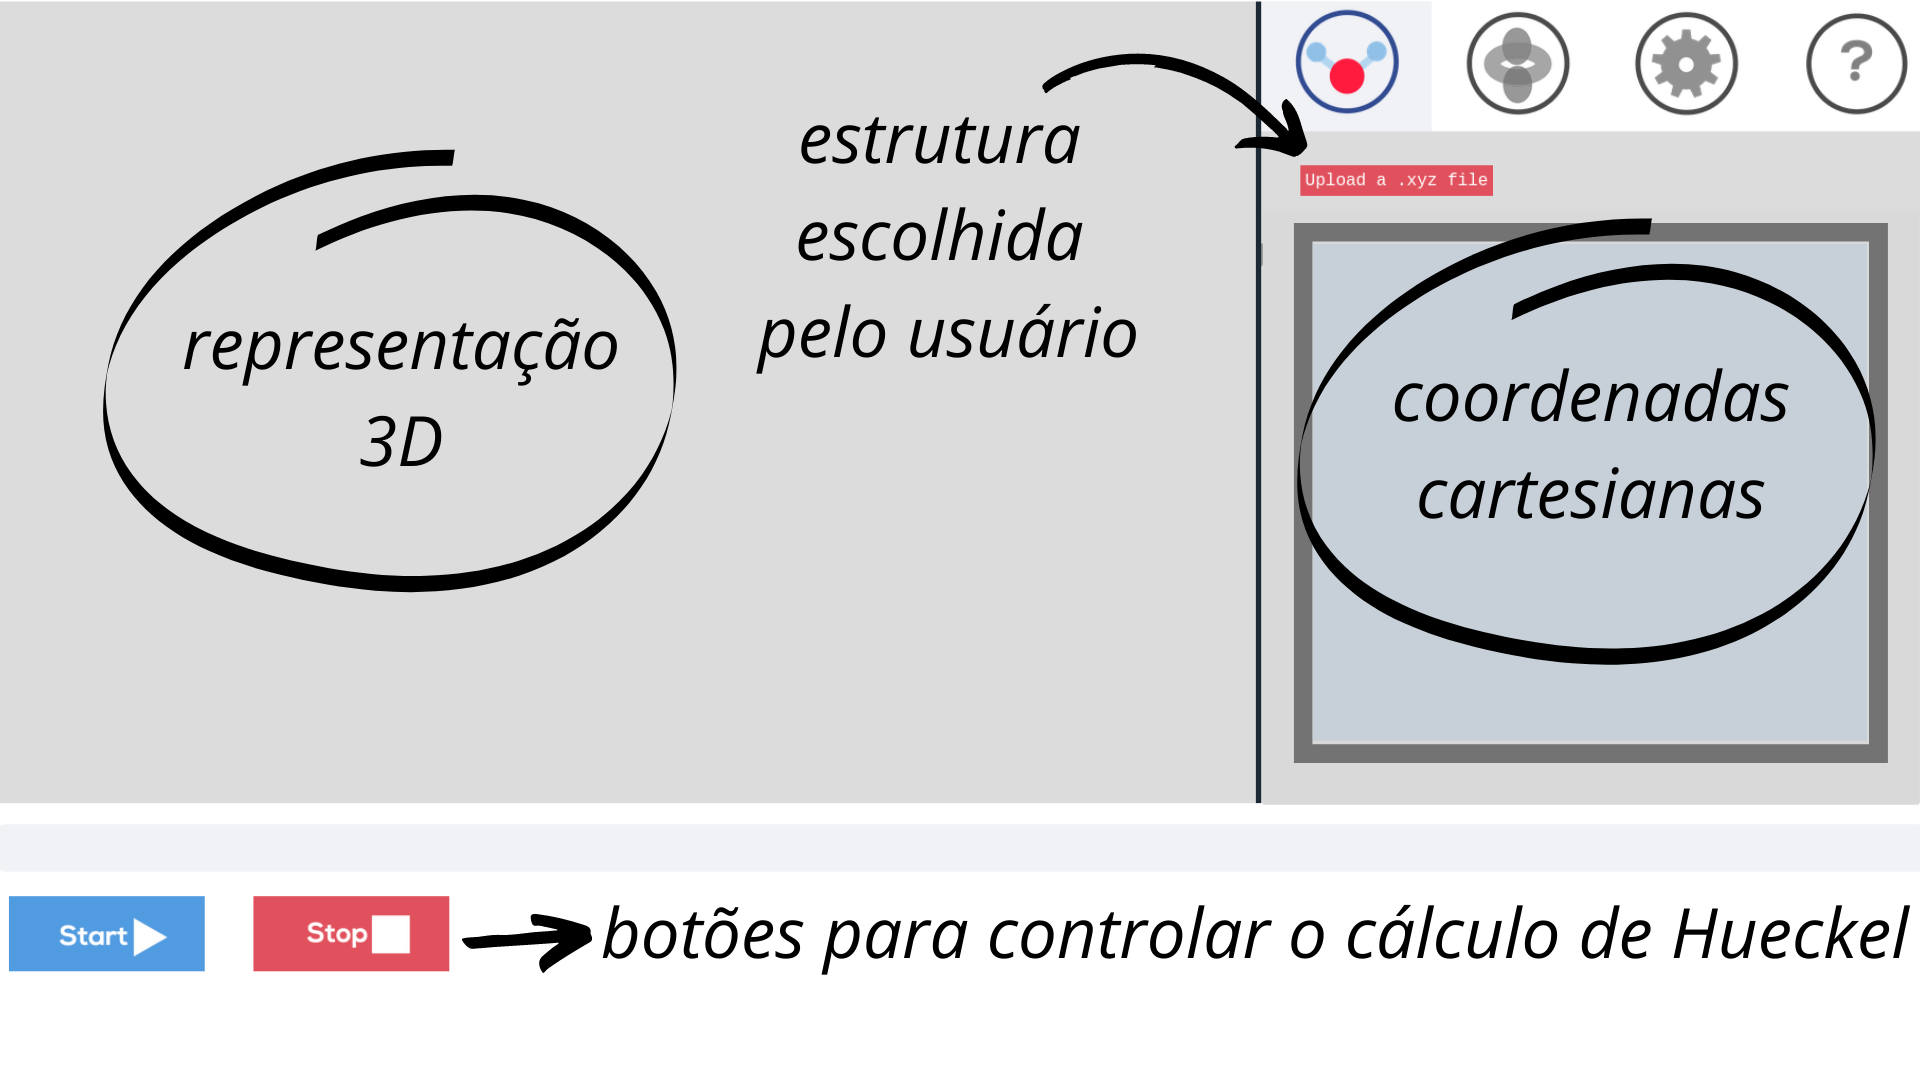
\includegraphics[width=0.8\textwidth]{images/GUI-EXAMPLE.png}
	\end{center}
	\fonte{Autor(a)}
\end{figure}

O fluxo de trabalho básico de funcionamento do \textit{Balmy.jl} também é ilustrado pelo esquema da \autoref{workflow}, onde é possível notar que o usuário insere, como entrada, o arquivo contendo as coordenadas cartesianas do sistema químico que deseja estudar. A \autoref{fig:input} mostra um exemplo de \textit{input} do \textit{Balmy.jl} para a molécula de benzeno. É um arquivo de extensão \textit{.xyz} que contém as coordenadas cartesianas da molécula de interesse. Na primeira linha, temos o nome da estrutura, em seguida, um comentário, e a partir da terceira linha são mostradas as informações da geometria em quatro colunas. A primeira delas contém os símbolos dos átomos contidos na molécula. Da segunda à quarta coluna, são indicadas as coordenadas cartesianas do eixo $x$, $y$ e $z$, respectivamente. Esses dados aparecem na caixa de texto no lado direito da tela (espaço indicado na \autoref{gui-pronta}).

\begin{figure}[htb]
	\caption{\label{fig:input} Exemplo de um arquivo de \textit{input} (\textit{.xyz}) para o \textit{Balmy.jl}.}
	\begin{center}
		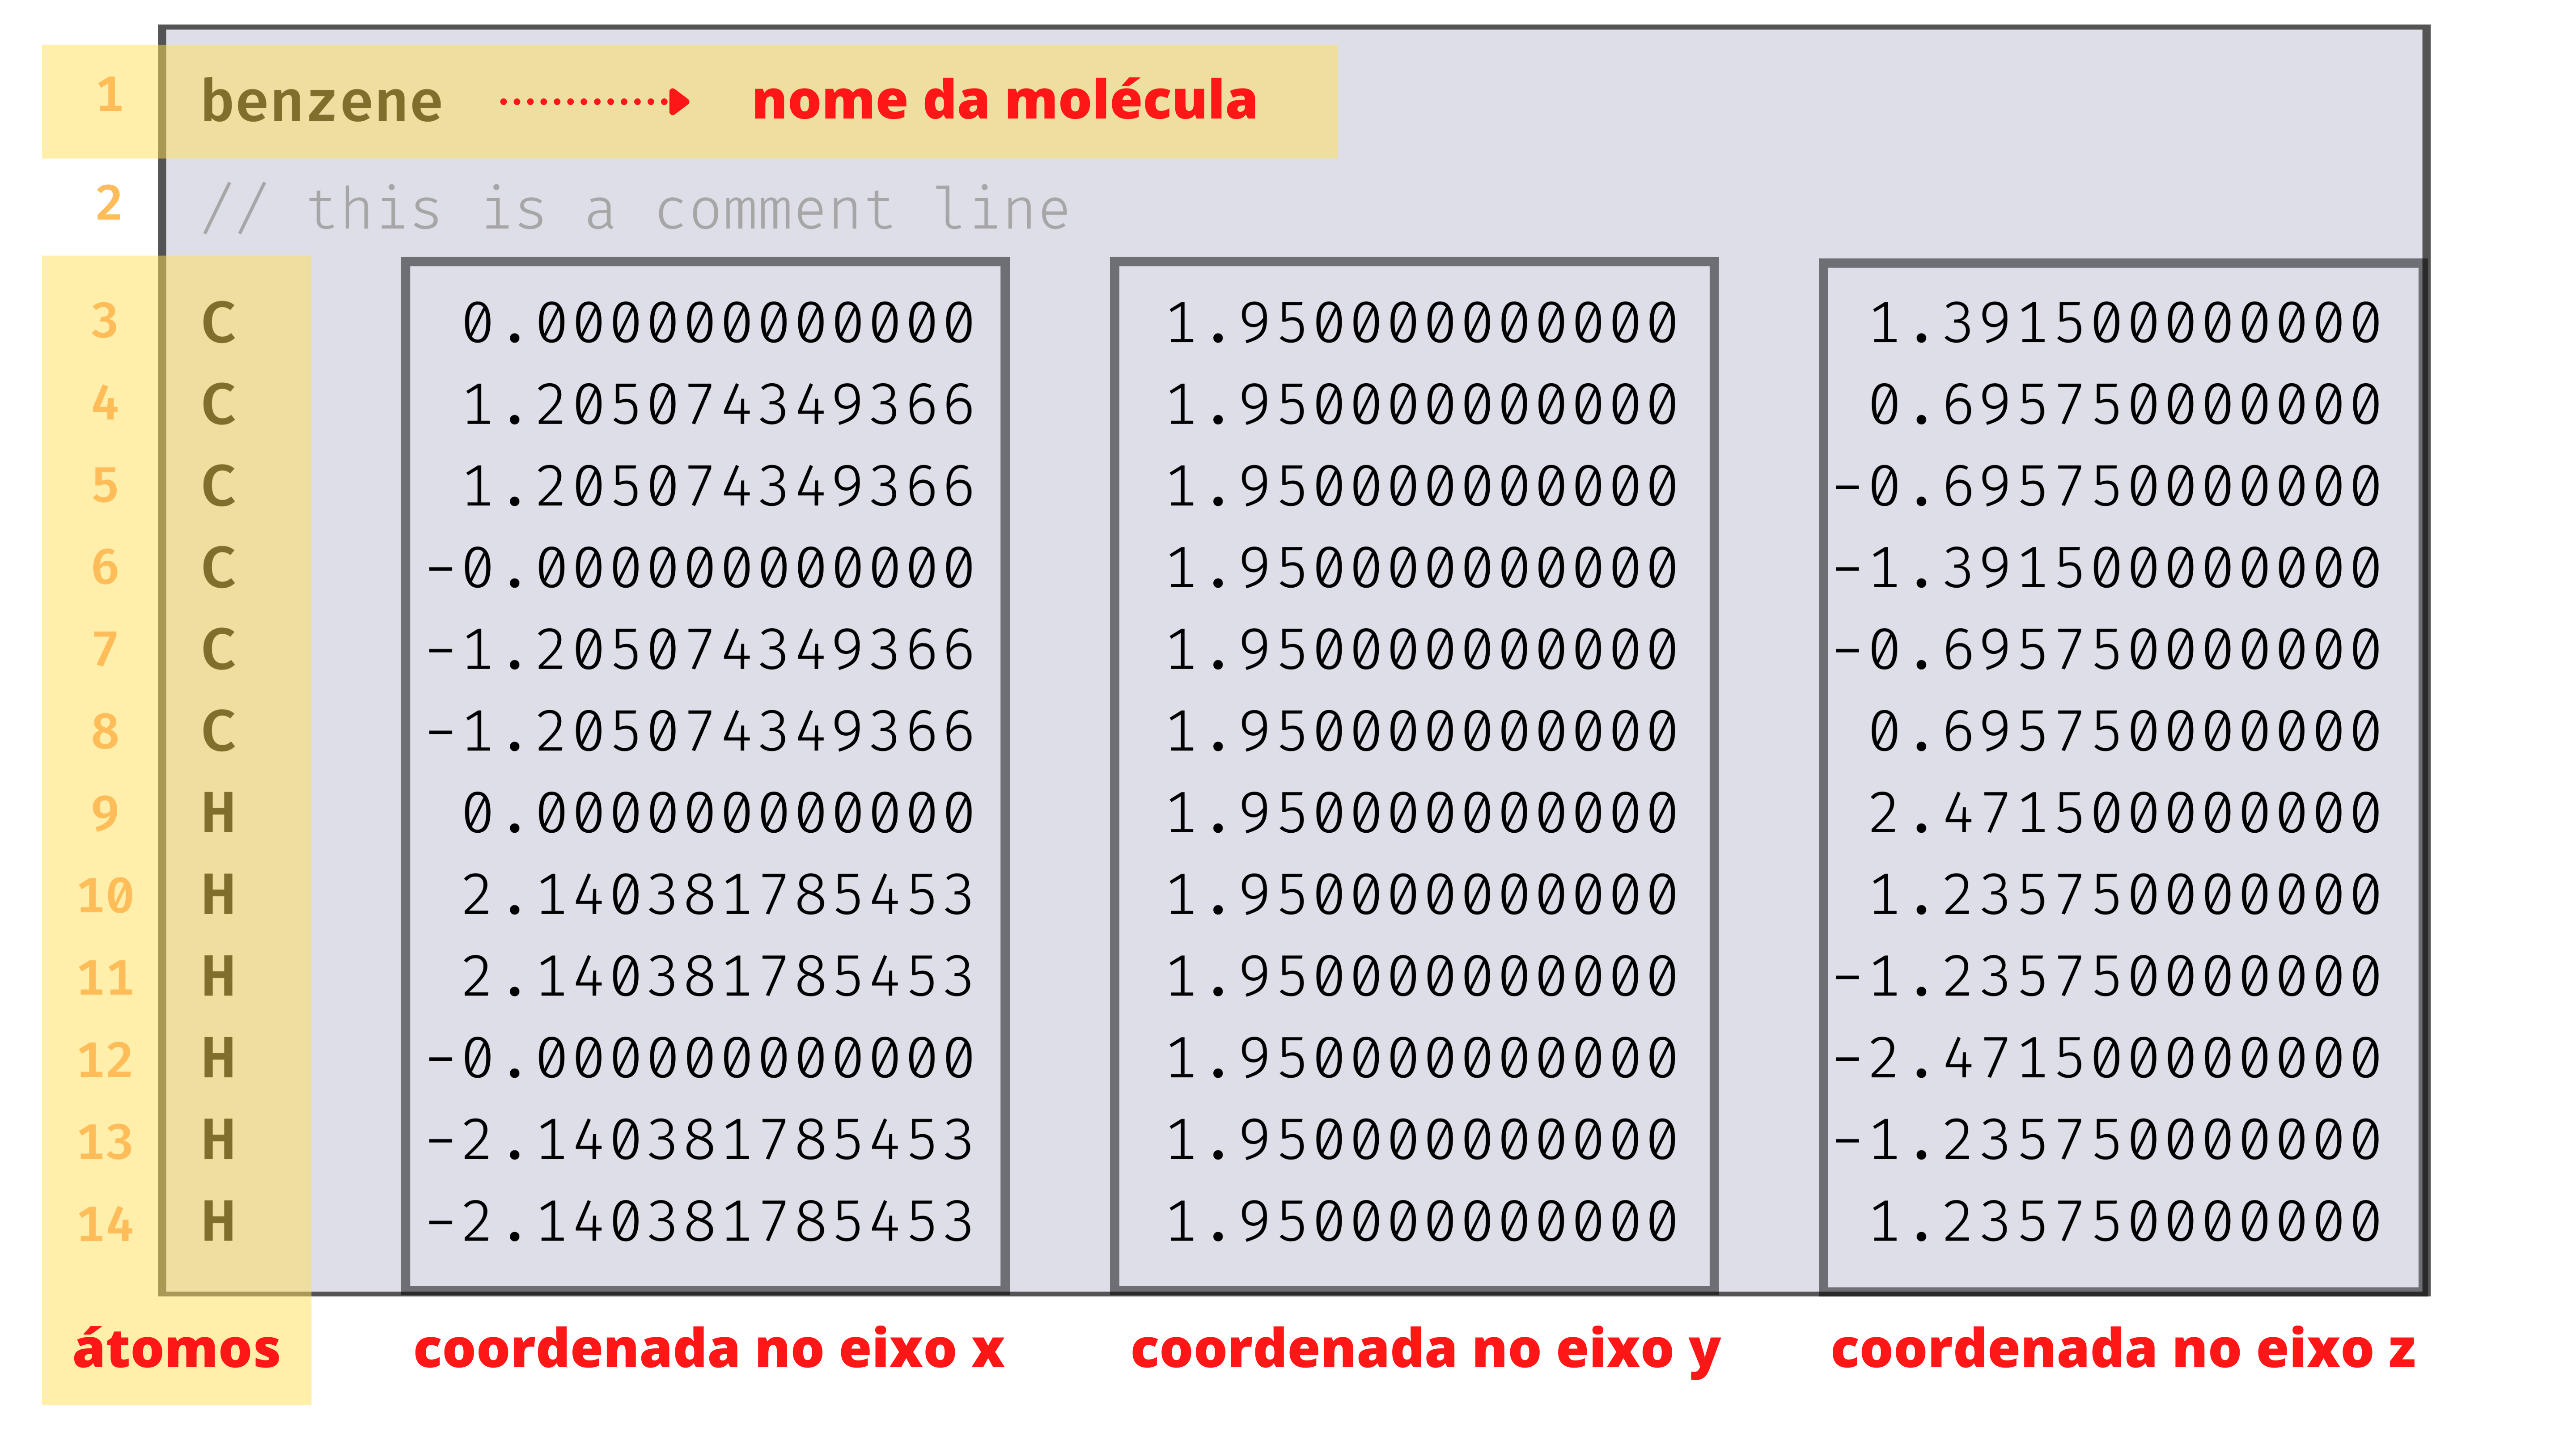
\includegraphics[width=0.8\textwidth]{images/fig2(4).png}
	\end{center}
	\fonte{Autor(a)}
\end{figure}

A partir das informações geométricas fornecidas pelo usuário, a estrutura é renderizada e representada tridimensionalmente pelo modelo das superfícies de Blinn-Phong (veja a \autoref{desenhoestrutural} para uma melhor descrição desse método). Nesse sentido, o \textit{Balmy.jl} é bastante versátil, pois é possível customizar o modelo através dos efeitos de iluminação empregados nas estruturas. Por exemplo, variando o valor de $\alpha'$ (coeficiente de brilho), é possível notar que, na \autoref{fig:representations}, quanto maior for o valor, menor será o holofote especular, representado pelos pontos luminosos nas estruturas moleculares.

%%% discutir equação do alpha

\begin{figure}[htb]
\caption{\label{fig:representations} Exemplo da aplicação do modelo de Blinn-Phong na molécula de benzenos a partir da alteração dos coeficientes $\alpha'$ para os átomos (representados por esferas). Da direita para a esquerda, os valores atribuídos foram: 0, 10, 50, 100, 1000; respectivamente.}
	\begin{center}
		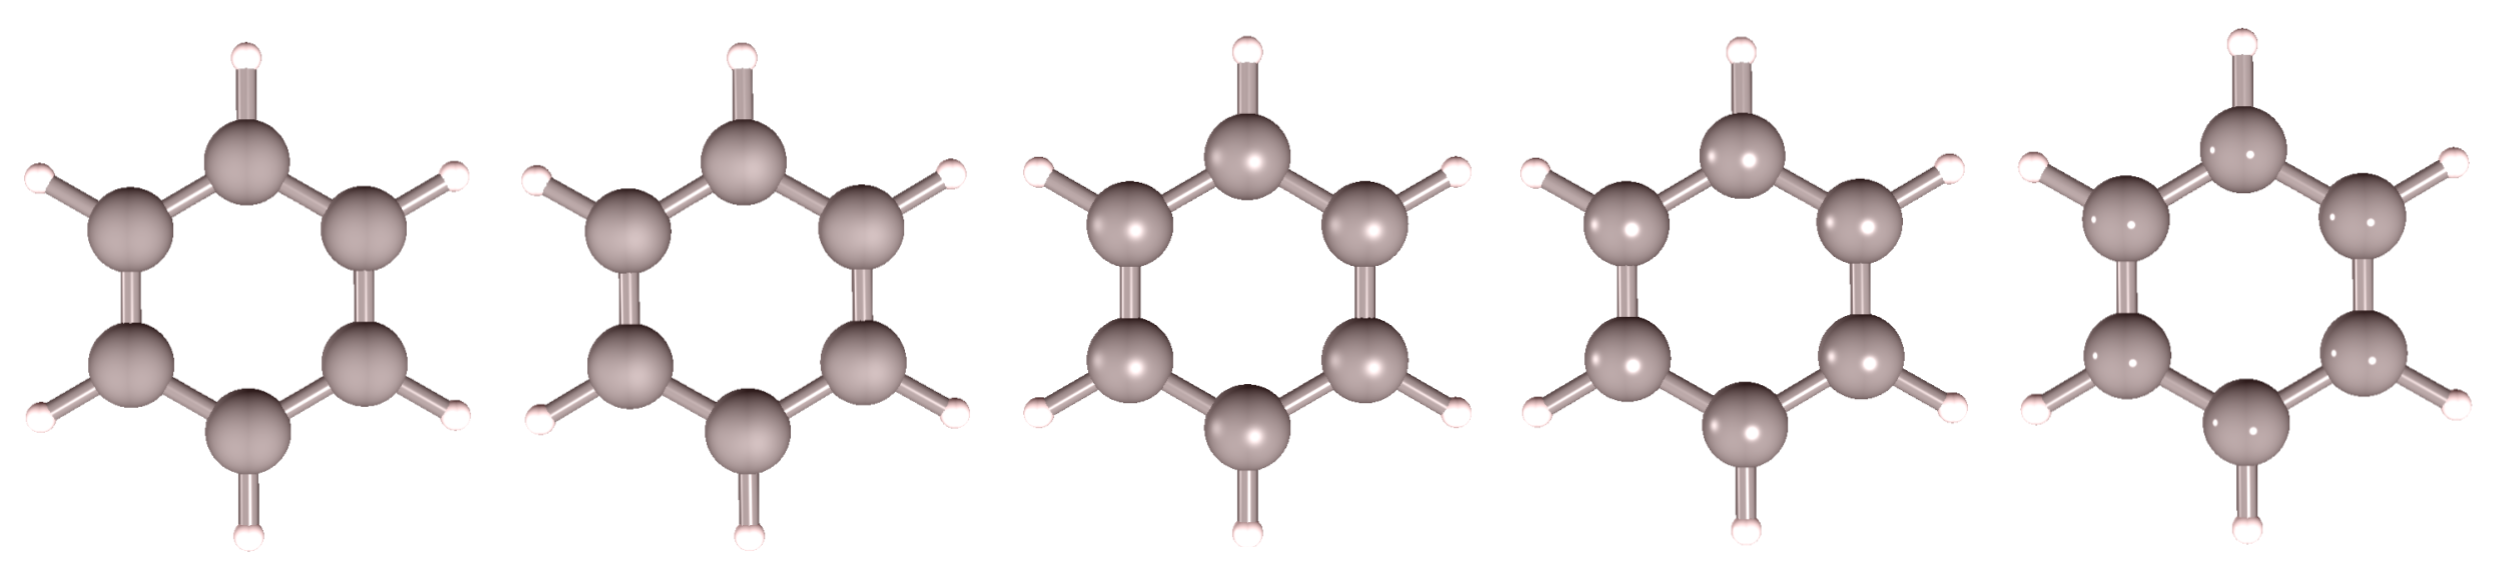
\includegraphics[width=1.0\textwidth]{images/shininess(1).png}
	\end{center}
	\fonte{Autor(a)}
\end{figure}

Antes da realização dos cálculos, é possível ainda acessar a terceira aba do \textit{Balmy.jl} para modificar o padrão das configurações (\autoref{fig:conf}). Por exemplo, é possível alterar a carga do composto (embora, por definição, o \textit{Balmy.jl} considere a moléula neutra) e o parâmetro de Wolfsberg-Helmholtz ($K$) (o padrão adotado é 1.75, parametrizado para hidrocarbonetos \autocite{Hoffmann1963}), que será discutido mais profundamente na \autoref{wolfsberg}.

\begin{figure}[htb]
	\caption{\label{fig:conf} Aqui, é mostrada a aba de configurações do cálculo realizado no \textit{Balmy.jl}}
	\begin{center}
		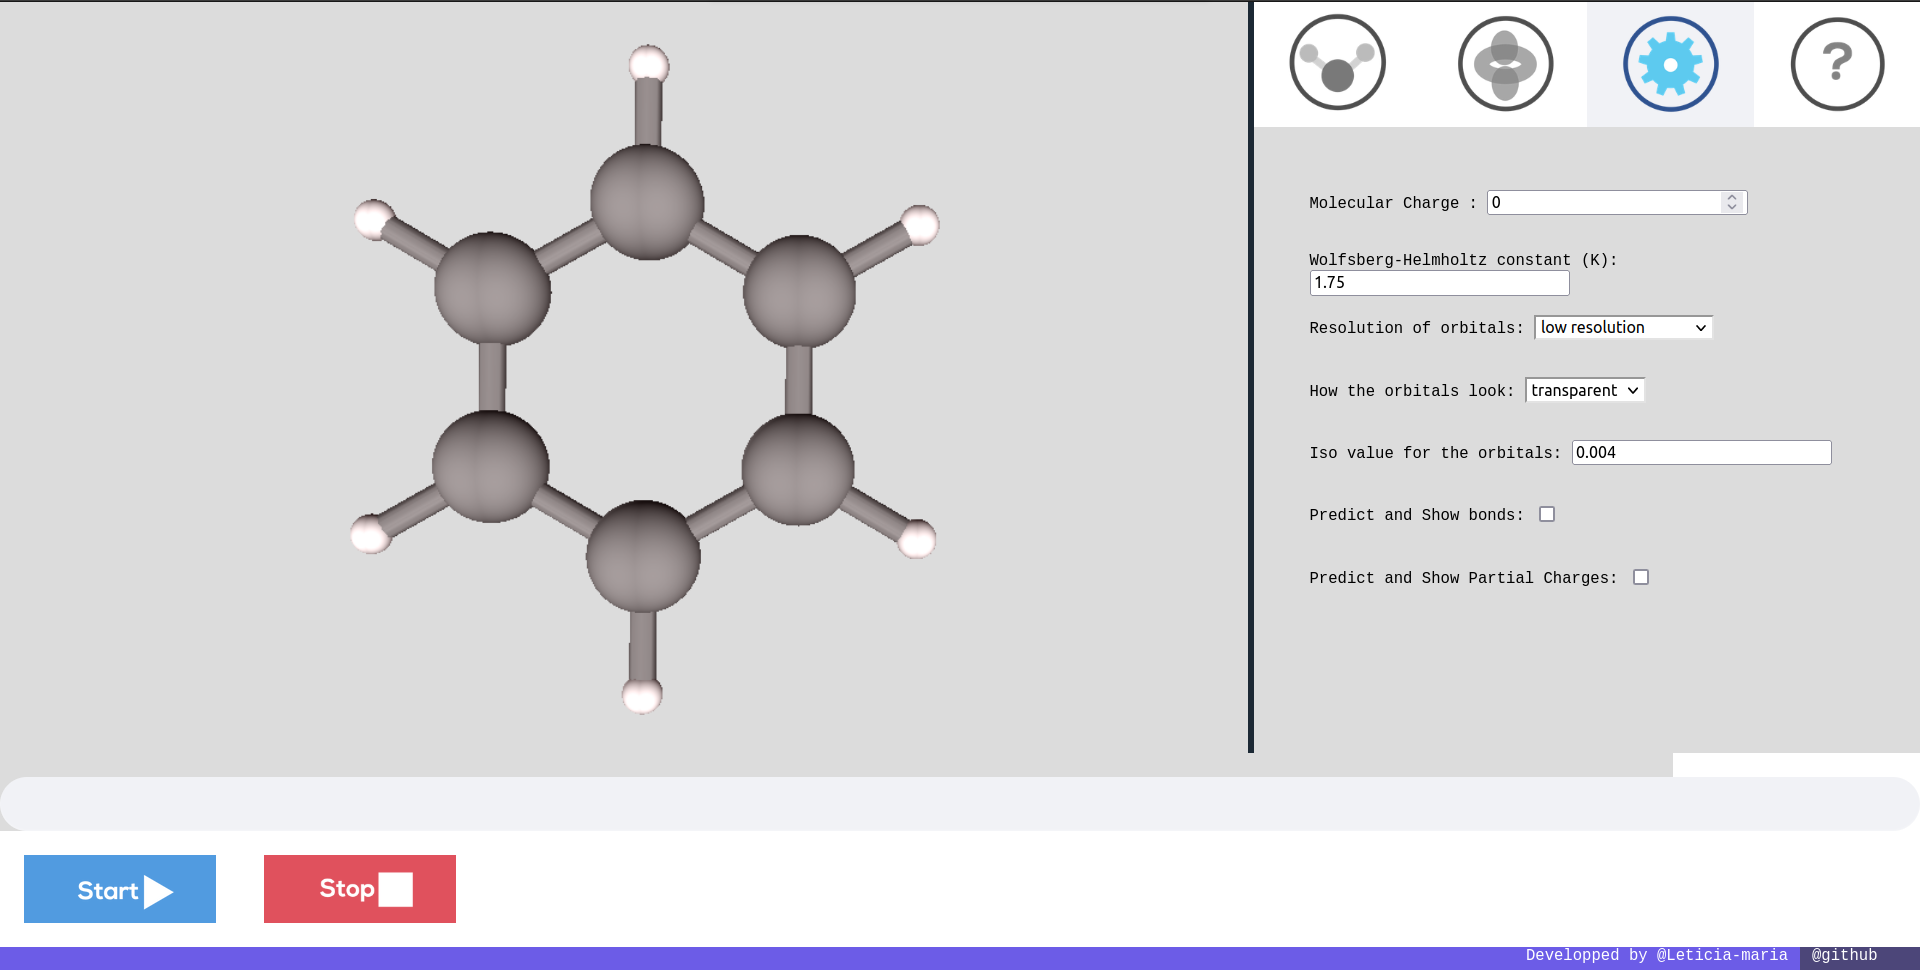
\includegraphics[width=0.8\textwidth]{images/conf.png}
	\end{center}
	\fonte{Autor(a)}
\end{figure}


Ao clicar no botão \textit{Start}, o usuário emite a requisição ao servidor para que o cálculo de \gls{EHMO} seja iniciado. Em questão de segundos, será possível acessar os resultados relativos ãs funções de onda e aos \gls{MOs} na segunda aba (\autoref{fig:results}). Para o caso do benzeno, os resultados serão discutidos na \autoref{sec:benzene}.

\begin{figure}[htb]
	\caption{\label{fig:results} Aqui, é mostrada a aba de resultados do cálculo realizado no \textit{Balmy.jl}}
	\begin{center}
		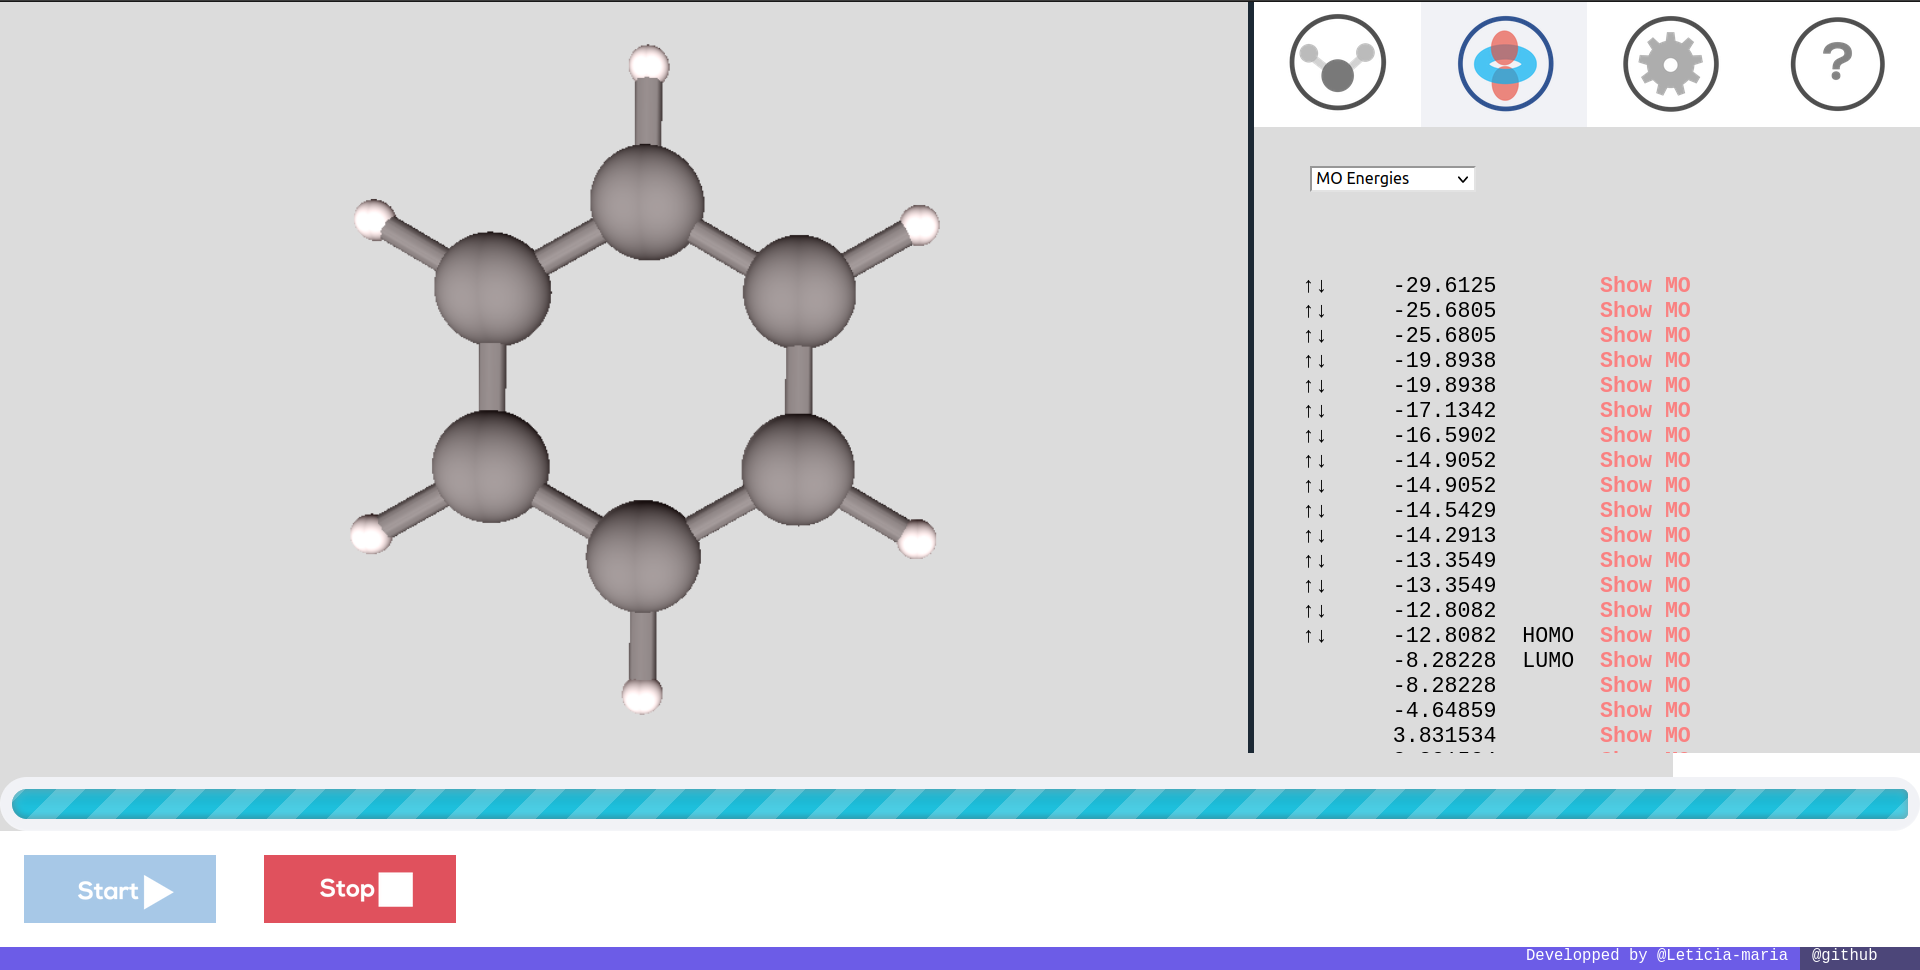
\includegraphics[width=0.8\textwidth]{images/results.png}
	\end{center}
	\fonte{Autor(a)}
\end{figure}

\section{Diagramas de orbitais moleculares}\label{sec:benzene}

Como o enfoque desse trabalho é a análise de compostos aromáticos, analisaremos de maneira mais aprofundada o exemplo do benzeno, cujas coordenadas estão mostradas na \autoref{tab:coords}. Os comprimentos de ligação obtidos para \ce{C-C} são $1.40$ \AA, e para \ce{C-H} são $1.10$ \AA.

\begin{table}[htb]
	\centering
	\caption{\label{tab:coords} Coordenadas atômicas do benzeno.}	
	\begin{tabular}{crrr}
		\toprule
		\textbf{Átomo (posição)} & coordenada $x$ & coordenada $y$ & coordenada $z$
		\\ 
		\midrule
C(1)  &    0.000000000000  &   1.950000000000  &   1.391500000000  \\
C(2)  &    1.205074349366  &   1.950000000000  &   0.695750000000  \\
C(3)  &    1.205074349366  &   1.950000000000  &  -0.695750000000  \\
C(4)  &   -0.000000000000  &   1.950000000000  &  -1.391500000000  \\
C(5)  &   -1.205074349366  &   1.950000000000  &  -0.695750000000  \\
C(6)  &   -1.205074349366  &   1.950000000000  &   0.695750000000  \\
H(1)  &    0.000000000000  &   1.950000000000  &   2.471500000000  \\
H(2)  &    2.140381785453  &   1.950000000000  &   1.235750000000  \\
H(3)  &    2.140381785453  &   1.950000000000  &  -1.235750000000  \\
H(4)  &   -0.000000000000  &   1.950000000000  &  -2.471500000000  \\
H(5)  &   -2.140381785453  &   1.950000000000  &  -1.235750000000  \\
H(6)  &   -2.140381785453  &   1.950000000000  &   1.235750000000  \\
    \bottomrule
	\end{tabular}
	\fonte{Autor(a).}
\end{table}

Seguindo o grafo mostrado na \autoref{fig:M2} e enumerado na \autoref{fig:graphEnumerated}, é possível construir uma matriz de adjacência de dimensão $n \times n$, onde $n$ é o número de átomos, excluindo-se os hidrogênios. No caso do benzeno, a ordem da matriz em questão é 6.

\begin{figure}[htb]
\vspace{0.8\baselineskip}
\begin{equation}
\label{eq:adjmatrix}
\begin{bmatrix}
    0 & 1 & 0 & 0 & 0 & 1 \\
    1 & 0 & 1 & 0 & 0 & 0 \\
    0 & 1 & 0 & 1 & 0 & 0 \\
    0 & 0 & 1 & 0 & 1 & 0 \\
    0 & 0 & 0 & 1 & 0 & 1 \\
    1 & 0 & 0 & 0 & 1 & 0
\end{bmatrix}
\end{equation}
\end{figure}

\noindent Consideremos $a_{ij}$ o elemento geral associado à matriz da \autoref{eq:5}, sendo igual a uma unidade quando os carbonos $i$ e $j$ estão ligados. Analogamente, na teoria de Hueckel e de Hueckel estendido, a matriz do determinante secular (\autoref{eq:secularmatrix}) é aquela cujos autovalores determinam as energias dos orbitais moleculares.

\begin{figure}[htb]
\vspace{0.8\baselineskip}
\begin{equation}
\label{eq:secularmatrix}
\begin{bmatrix}
    \alpha - E & \beta & 0 & 0 & 0 & \beta \\
    \beta & \alpha - E & \beta & 0 & 0 & 0 \\
    0 & \beta & \alpha - E & \beta & 0 & 0 \\
    0 & 0 & \beta & \alpha - E & \beta & 0 \\
    0 & 0 & 0 & \beta & \alpha - E & \beta \\
    \beta & 0 & 0 & 0 & \beta & \alpha - E \\
\end{bmatrix}
\end{equation}
\end{figure}

No caso do benzeno, ao resolver o determinante secular da matriz anterior (através do procedimento mostrado no \autoref{ap:HMO} e no \autoref{ap:EHMO}), obtemos a equação

\begin{figure}[htb]
\begin{equation}
    \label{eq:R3}
    \tikzmarknode{variable}{\highlight{blue}{$x$}}^6 - 6\highlight{blue}{$x$}^4 + 9\highlight{blue}{$x$}^2 = 0
\end{equation}
\begin{tikzpicture}[overlay,remember picture,>=stealth,nodes={align=left,inner ysep=1pt},<-]
    \path (variable.south) ++ (1,-1.5em) node[anchor=north west,color=blue!67] (scalep){\textit{$x = \displaystyle \frac{\alpha - E}{\beta}$}};
    \draw [color=blue!87](variable.south) |- ([xshift=1.65em,color=blue]scalep.north east);
\end{tikzpicture}
\vspace{2\baselineskip}
\end{figure}

\begin{figure}[htb]
\vspace{2\baselineskip}
\begin{equation}
    \label{eq:orb_mols}
\begin{split}
    \tikzmarknode{e1}{\highlight{blue}{$E_1$}} = \alpha +  2 \beta \\[0.3cm]
    \tikzmarknode{e2}{\highlight{red}{$E_2 = E_3$}} = \alpha + \beta \\
    \tikzmarknode{e3}{\highlight{red}{$E_4 = E_5$}} = \alpha - \beta \\[0.3cm]
    \tikzmarknode{e6}{\highlight{blue}{$E_6$}} = \alpha - 2\beta
\end{split}
\end{equation}
\begin{tikzpicture}[overlay,remember picture,>=stealth,nodes={align=left,inner ysep=1pt},<-]
    \path (e1.north) ++ (1,1.5em) node[anchor=south west,color=blue!67] (scalep){\textit{HOMO-1}};
    \draw [color=blue!87](e1.north) |- ([xshift=1.65em,color=blue]scalep.south east);

    \path (e2.north) ++ (-0.60,0.6em) node[anchor=south east,color=red!67] (scalep){\textit{HOMO (orbitais degenerados)}};
    \draw [color=red!87](e2.north) |- ([xshift=-1.65em,color=red]scalep.south west);
    
    \path (e3.south) ++ (-0.60,-0.6em) node[anchor=north east,color=red!67] (scalep){\textit{LUMO (orbitais degenerados)}};
    \draw [color=red!87](e3.south) |- ([xshift=-1.65em,color=red]scalep.north west);
    
    \path (e6.south) ++ (1,-1.5em) node[anchor=north west,color=blue!67] (scalep){\textit{LUMO+1}};
    \draw [color=blue!87](e6.south) |- ([xshift=1.65em,color=blue]scalep.north east);
\end{tikzpicture}
\end{figure}

Resolvendo o polinômio da \autoref{eq:R3}, conseguimos suas raízes ($x = \pm 1, \pm 1, \pm 2$) e, portanto, as energias para seis orbitais moleculares do benzeno (HOMO-1, HOMO, LUMO, LUMO+1). Combinando as raízes com os parâmetros $\alpha$ e $\beta$, nós temos a \autoref{eq:orb_mols} (\autoref{fig:MOs}).

\begin{figure}[htb]
\caption{\label{fig:MOs} Diagrama de energia dos orbitais moleculares do benzeno.}
	\begin{center}
		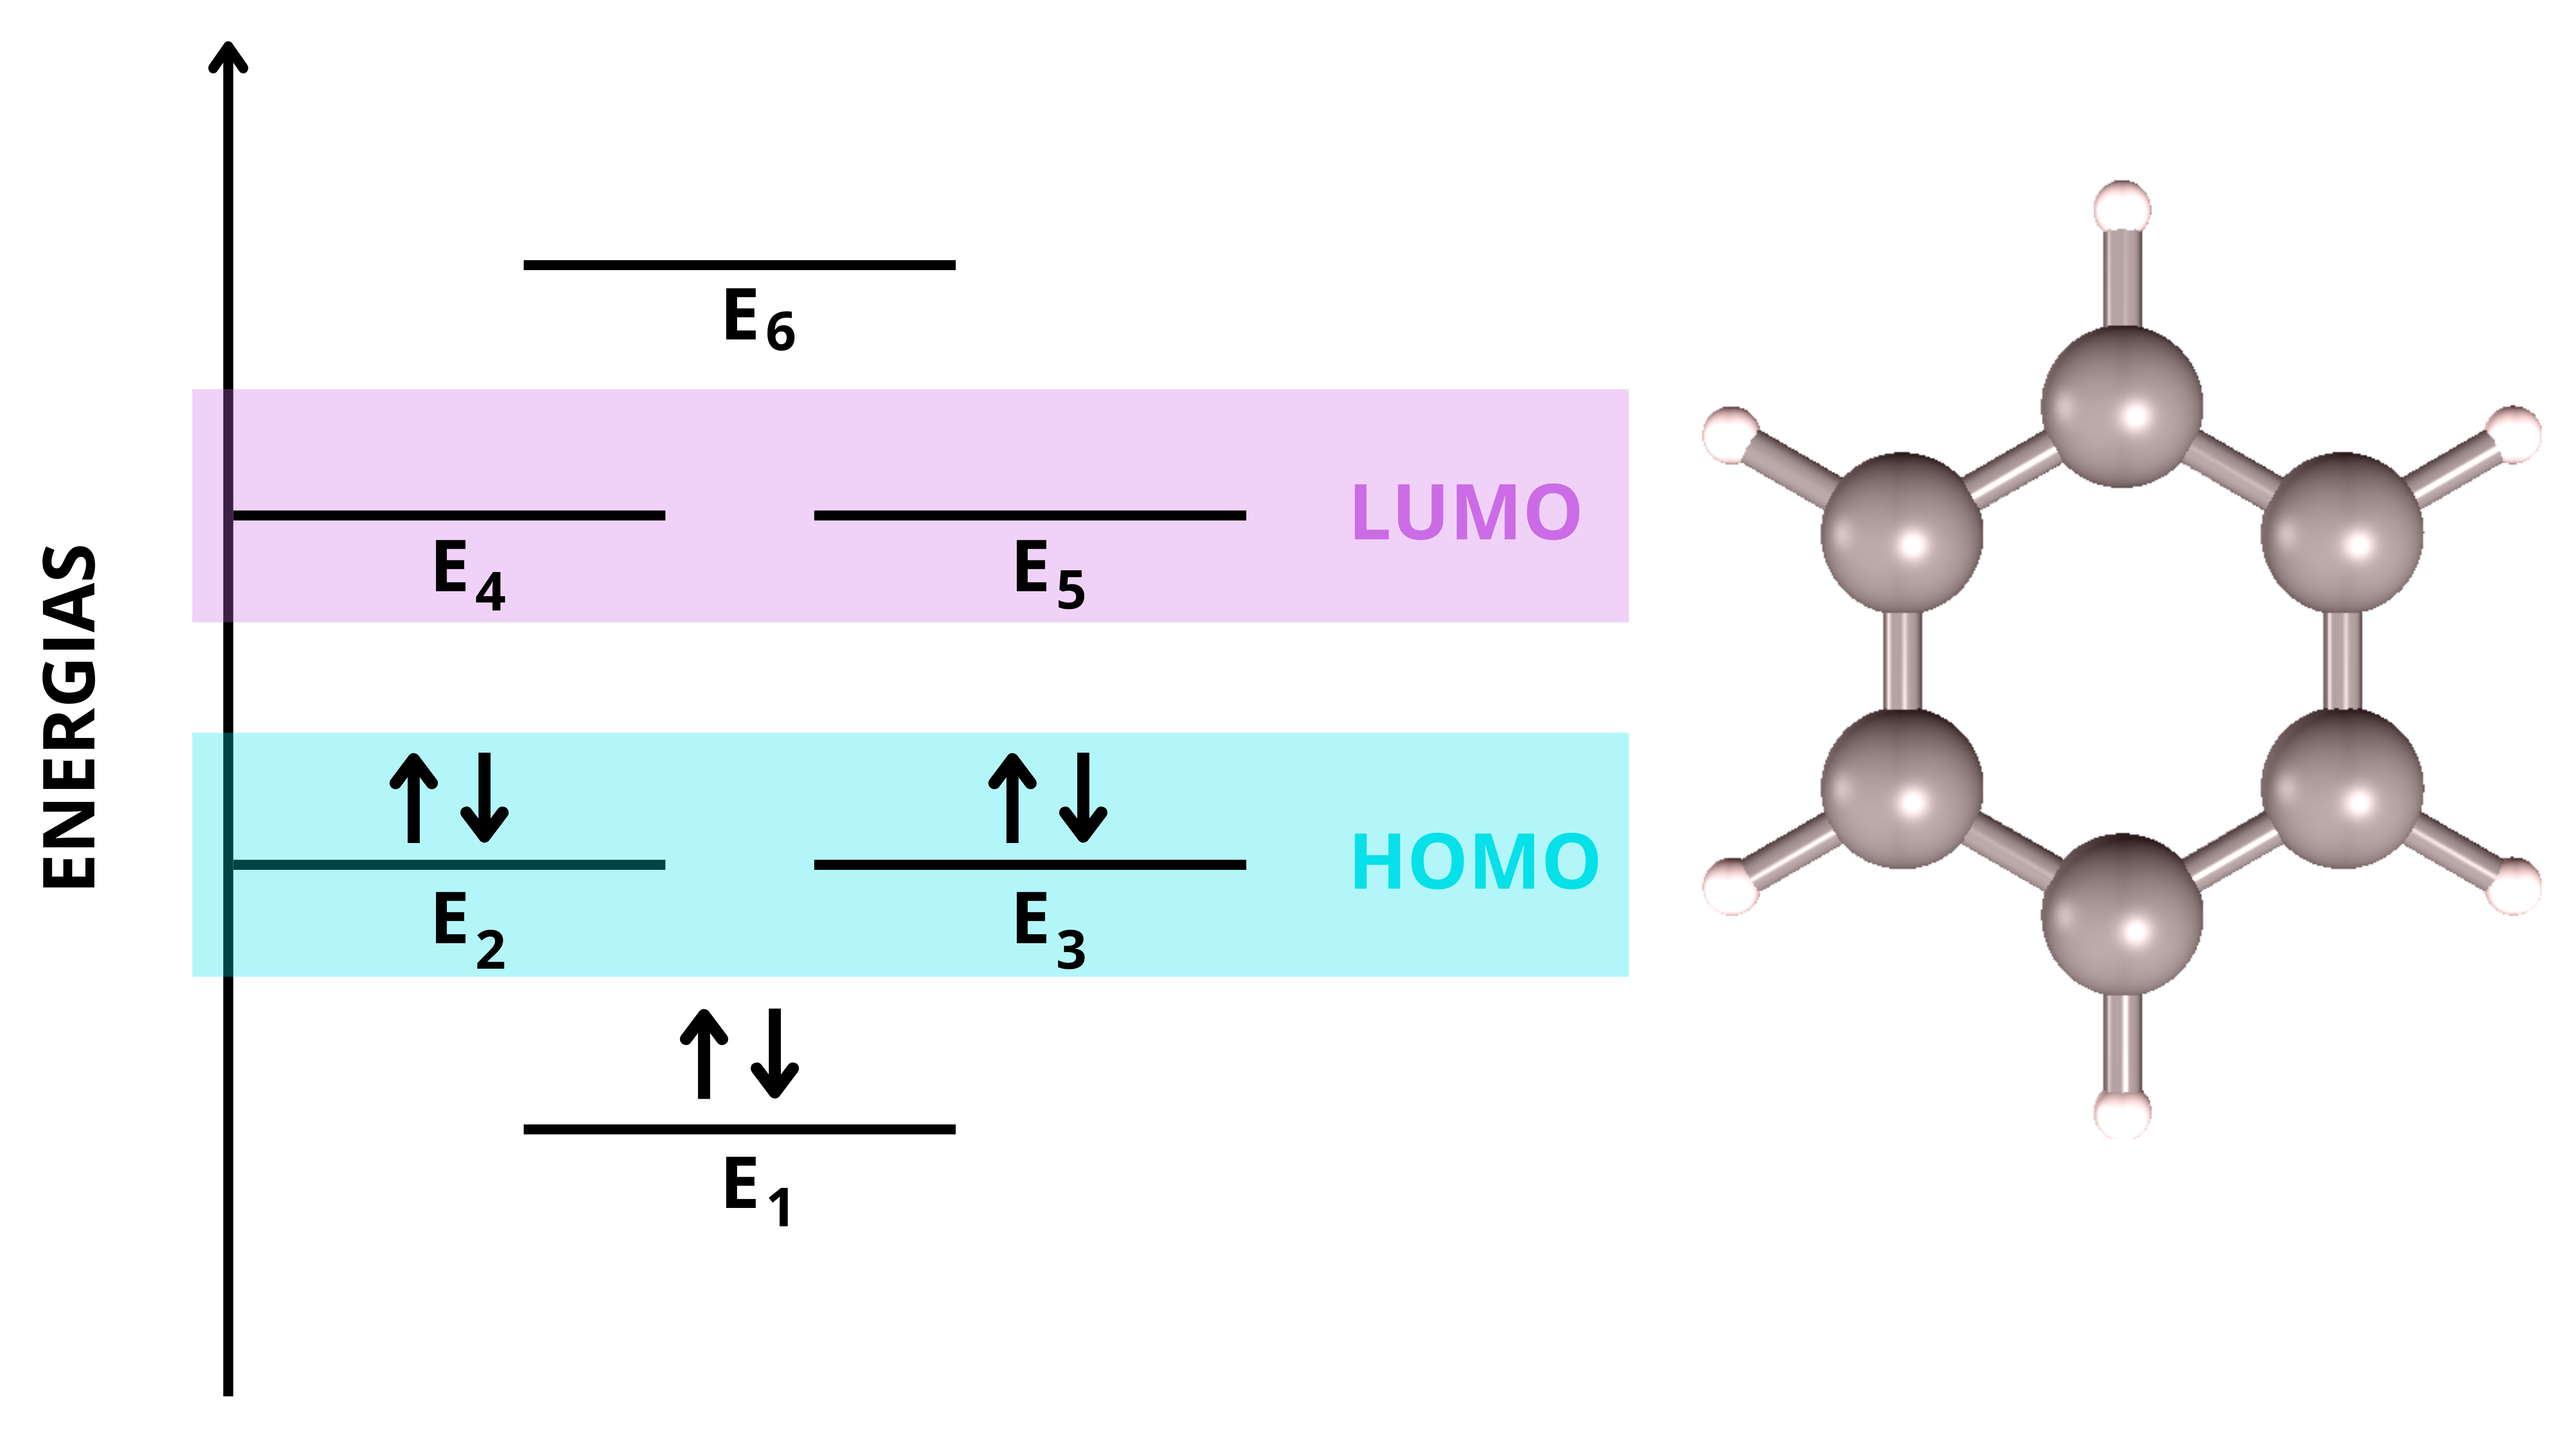
\includegraphics[width=0.75\textwidth]{images/MOs.png}
	\end{center}
	\fonte{Autor(a).}
\end{figure}

Os autovalores repetidos vão gerar orbitais degenerados, isto é, aqueles que estão no mesmo nível energético, como é possível notar no diagrama e nos valores de energia obtidos. Esses mesmos valores podem ser obtidos se calcularmos os autovalores da matriz de adjacência. Desse modo, comprovamos que, ao solucionar o determinante e os autovalores da matriz secular, é possível obter os valores de energia e as populações associadas a cada orbital molecular da molécula de interesse.

O diagrama de níveis de energia para o benzeno é dado na \autoref{fig:MOs}. Os seis elétrons $\pi$ são colocados nos três níveis de energia mais baixos. Desse modo, a energia eletrônica em benzeno é definida pela \autoref{epi}.

\begin{equation}
\label{epi}
    E_\pi = 2(\alpha + 2\beta) + 4(\alpha + \beta) = 6\alpha + 8\beta
\end{equation}

As funções de onda resultantes para os seis orbitais moleculares $\pi$ do benzeno são dados pela \autoref{wavefunctions}.

\begin{equation}
\label{wavefunctions}
\begin{split}
    \psi_1 = \frac{1}{\sqrt{6}}(2p_{z1} + 2p_{z2} + 2p_{z3} + 2p_{z4} + 2p_{z5} + 2p_{z6}) \Longrightarrow E_1 = \alpha + 2\beta \\
    \psi_2 = \frac{1}{\sqrt{4}}(2p_{z2} + 2p_{z3} - 2p_{z5} - 2p_{z6}) \Longrightarrow E_2 = \alpha + \beta \\
   \psi_3 = \frac{1}{\sqrt{3}}(2p_{z1} + \frac{1}{2} 2p_{z2} - \frac{1}{2} 2p_{z3} - 2p_{z4} - \frac{1}{2} 2p_{z5} + \frac{1}{2} 2p_{z6}) \Longrightarrow E_3 = \alpha + \beta \\
     \psi_4 = \frac{1}{\sqrt{4}}(2p_{z2} - 2p_{z3} + 2p_{z5} - 2p_{z6}) \Longrightarrow E_4 = \alpha - \beta \\
      \psi_5 = \frac{1}{\sqrt{3}}(2p_{z1} - \frac{1}{2} 2p_{z2} - \frac{1}{2} 2p_{z3} + 2p_{z4} - \frac{1}{2} 2p_{z5} - \frac{1}{2} 2p_{z6}) \Longrightarrow E_5 = \alpha - \beta \\
      \psi_6 = \frac{1}{\sqrt{6}}(2p_{z1} - 2p_{z2} + 2p_{z3} - 2p_{z4} +  2p_{z5} -  2p_{z6}) \Longrightarrow E_6 = \alpha - 2\beta 
\end{split}
\end{equation}


\begin{table}[htb]
	\centering
	\caption{\label{qua:Quadro_1} Energias dos orbitais de fronteira de alguns hidrocarbonetos aromáticos.}	
	\begin{tabular}{lrrr}
		\toprule
		\textbf{Molécula} & \textbf{HOMO/(eV)} & \textbf{LUMO/(eV)} & \textbf{Gap/(eV)}
		\\ 
		\midrule
        benzeno & -12.808 & -8.282 & 4.452 \\
        naftaleno & -12.073 & -9.338 & 2.635 \\
        antraceno & -11.642 & -9.839 & 1.803 \\
        fenantreno & -12.023 & -9.310 & 2.713 \\
        azuleno & -11.730 & -9.872 & 1.858 \\
        pentaleno & -11.492 & -10.809 & 0.683 \\
        fulveno & -11.991 & -10.338 & 1.653 \\
        bifenileno & -11.555 & -9.553 & 2.002 \\
        tolueno & -12.502 & -8.348 & 4.154 \\
    \bottomrule
	\end{tabular}
	\fonte{Autor(a).}
\end{table}

\section{Hidrocarbonetos aromáticos}

Analisando os dados da \autoref{tab:energies}, concluímos que a ordem das estabilidades dos compostos está de acordo com aqueles apresentados por Hoffmann \autocite{Hoffmann1963}, e com os dados experimentais publicados por Heilbronner \autocite{ginsburg1959}. Por exemplo, o naftaleno mostra-se 32.3 kcal/mol mais estável do que o azuleno, o que é um ótimo resultado se comparado com o valor de referência (32.6 kcal/mol)\autocite{ginsburg1959}. O fulveno, por sua vez, é computado como sendo 25.6 kcal/mol menos estável do que o benzeno, em relação ao valor de 27 kcal/mol tomado como modelo\autocite{CHENG1956}. O antraceno, por sua vez, é 4.2 kcal/mol mais estável do que o fenantreno, enquanto o último isômero é, na verdade, 6.9 kcal/mol mais estável \autocite{Hoffmann1963}, o que provém do fato de que há repulsão estérica entre os hidrogênios do fenantreno.

\begin{table}[htb]
	\centering
	\caption{\label{tab:energies} Energias dos elétrons $\pi$ nos compostos aromáticos.}	
	\begin{tabular}{lrr}
		\toprule
		\textbf{Molécula} & $E_\pi / (eV)$ & $E_\pi / (kcal/mol)$
		\\ 
		\midrule
        Etileno & -26.336 & -609.628 \\
        Butadieno & -52.964 & -1221.38 \\
        Benzeno & -80.208 & -1849.64 \\
        Fulveno & -78.928 & -1820.12 \\
        Naftaleno & -133.676 & -3082.64 \\
        Azuleno & -132.934 & -3065.53 \\
        Fenantreno & -187.286 & -4318.92 \\
        Antraceno & -187.020 & -4312.78 \\
    \bottomrule
	\end{tabular}
	\fonte{Autor(a).}
\end{table}

\section{Influência de K}\label{wolfsberg}


\section{Performance}


\newpage

\section{Índices geométricos}

Além dos orbitais moleculares e das funções de onda, o \textit{Balmy.jl} também permite analisar o \gls{HOMA}. Esse índice geométrico de aromaticidade foi modelado de acordo com uma escala normalizada pelo fator $\alpha$ (\autoref{eq:3}), onde o benzeno seria a referência de \textit{aromaticidade perfeita}, tendo \gls{HOMA} $=1$, pois o desvio entre os comprimentos de ligação individuais ($R_i$) e o comprimento ótimo de ligação ($R_{opt}$) (\autoref{eq:2}) é nulo. Isso faz com que os termos $EN$ e $GEO$, que diminuem a aromaticidade, sejam iguais a $0$.

\begin{equation}
    HOMA = 1 - EN - GEO \Longrightarrow HOMA = 1 - 0 - 0 \Longrightarrow HOMA = 1
\end{equation}

\begin{table}[htb]
	\centering
	\caption{\label{tab:ccbc} Comprimentos de ligação entre átomos de carbono. Como notação, adotamos a simbologia \ce{C-C} para representar a ligação simples, \ce{C=C} para a ligação dupla, \ce{C\simeq C} para representar a ligação CC aromática na molécula do benzeno.}	
	\begin{tabular}{ccc}
		\toprule
		\textbf{Tipo de ligação} & \textbf{Energia de ligação} & \textbf{Comprimento de ligação} \\
		\midrule
         \ce{C-C}  & 345 kJ/mol & 1.53 \AA \\
         \ce{C=C} & 612 kJ/mol & 1.34 \AA \\
         \ce{C\simeq C} & 420 kJ/mol & 1.40 \AA \\
    \bottomrule
	\end{tabular}
	\fonte{Autor(a).}
\end{table}

Por outro lado, \gls{HOMA} $= 0$ para o cicloexatrieno hipotético (\autoref{fig:2}), composto por ligações simples e duplas, sem deslocalização. Pode-se facilmente deduzir isso através da substituição dos valores da \autoref{tab:ccbc} na \autoref{eq:4}.

\begin{equation}
    \begin{split}
        HOMA = 1 - \bigg\{ \frac{98.89}{6} \{ 3[(1.40 - R_{\ce{C-C}})^2] + 3[(1.40 - R_{\ce{C=C}})^2] \} \bigg\} \\
        HOMA = 1 - \bigg\{ \frac{98.89}{6} \{ 3[(1.40 - 1.53)^2] + 3[(1.40 - 1.34)^2] \} \bigg\} \\
        HOMA = 1 - \bigg[ \frac{98.89}{6} (0.0615) \bigg] \\
        HOMA = 1 - 1 = 0
    \end{split}
\end{equation}

%Ou seja, a ideia original e fundamental é que cada par de átomos pode ser envolvido em ambas as ligações $\sigma$ e $\pi$, com $R_\sigma > R_\pi$. A distância de ligação $R_i$ representa uma compressão de $R_\sigma$ e uma extensão de $R_\pi$.

\subsection{Hidrocarbonetos policíclicos aromáticos}

O arquivo de saída gerado pelo \textit{Balmy.jl} para o usuário analisar e visualizar essas relações está representado na \autoref{fig:HOMA}. Para explorar um pouco mais a importância do \gls{HOMA}, o índice foi aplicado a alguns sistemas policíclicos aromáticos. Ao observar os valores na \autoref{fig:HOMA}, nota-se que os sextetos mais aromáticos estão na região perférica mais externa (\gls{HOMA} $= 0.9$), o que é um fenômeno importante, pois o \gls{HOMA} conhecidamente superestima os valores de aromaticidade para sextetos periféricos\autocite{giov2020}. 

\begin{figure}[htb]
\caption{\label{fig:HOMA} Valores de HOMA para a estrutura do Kekuleno gerados com o \textit{Balmy.jl}.}
	\begin{center}
		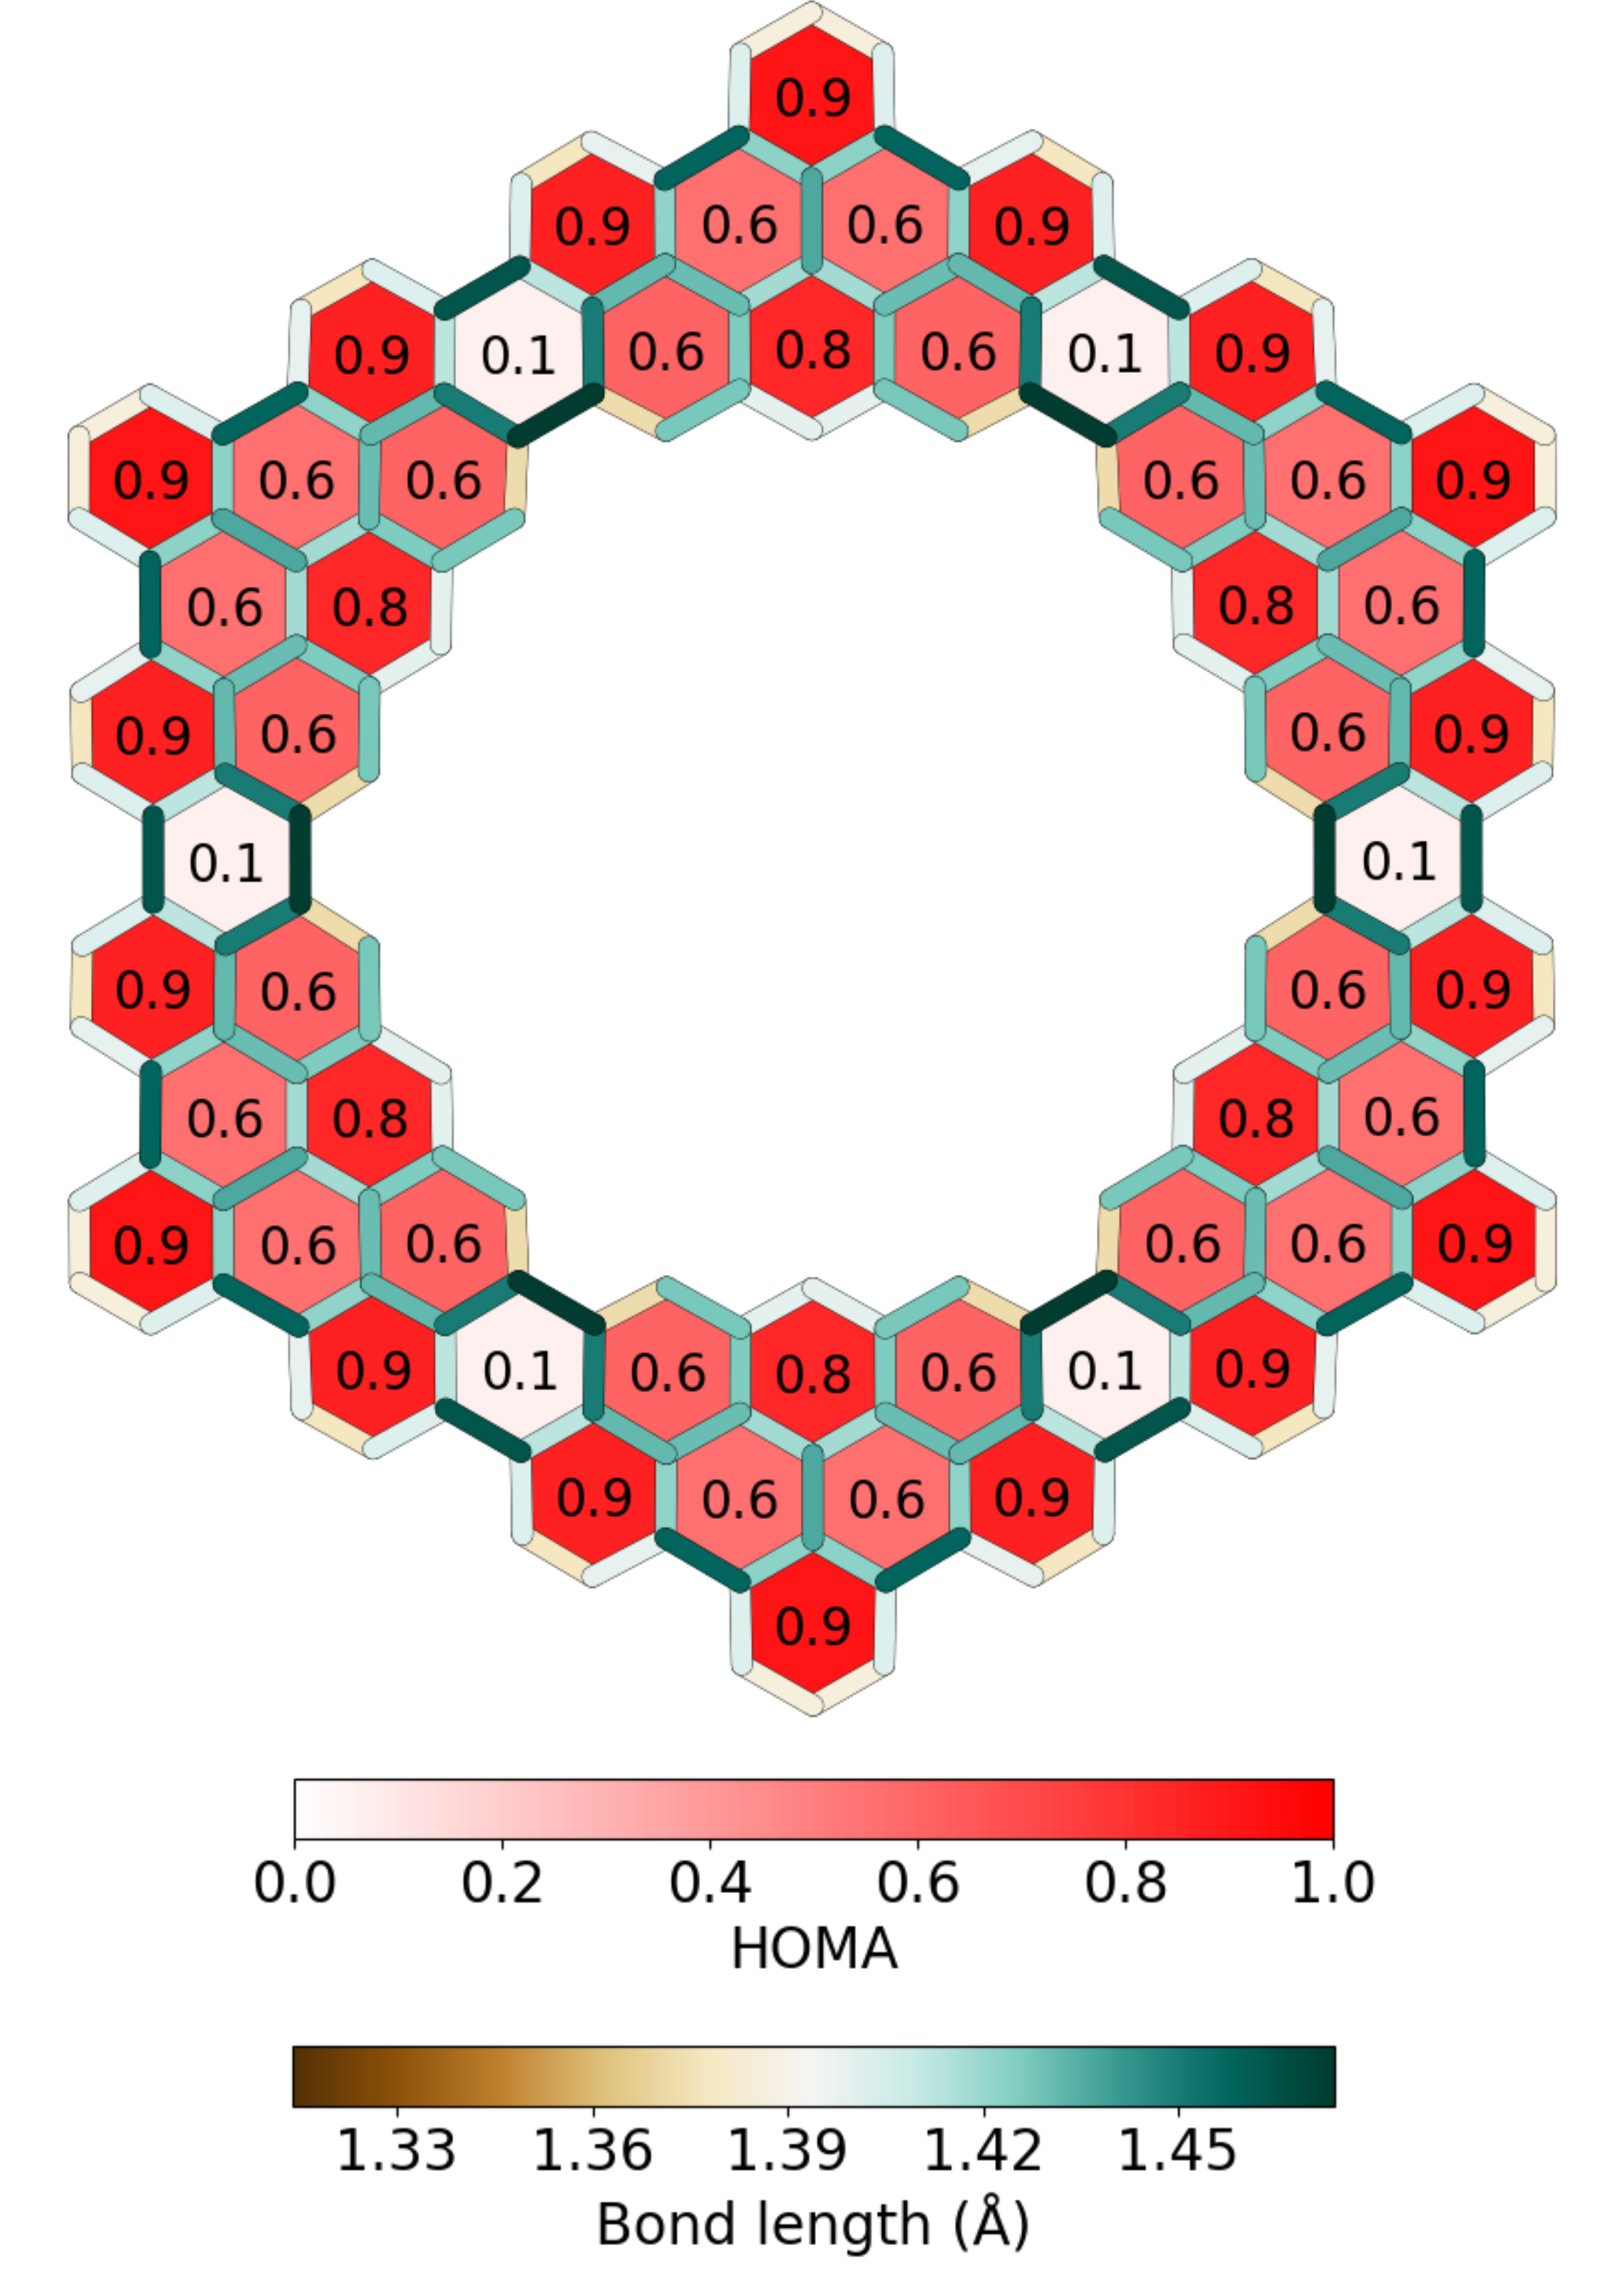
\includegraphics[width=0.65\textwidth]{images/geom.png}
	\end{center}
	\fonte{Autor(a).}
\end{figure}

\begin{figure}[htb]
\caption{\label{fig:HOMA2} Valores de HOMA para a estrutura do Kekuleno gerados com o \textit{Balmy.jl}.}
	\begin{center}
		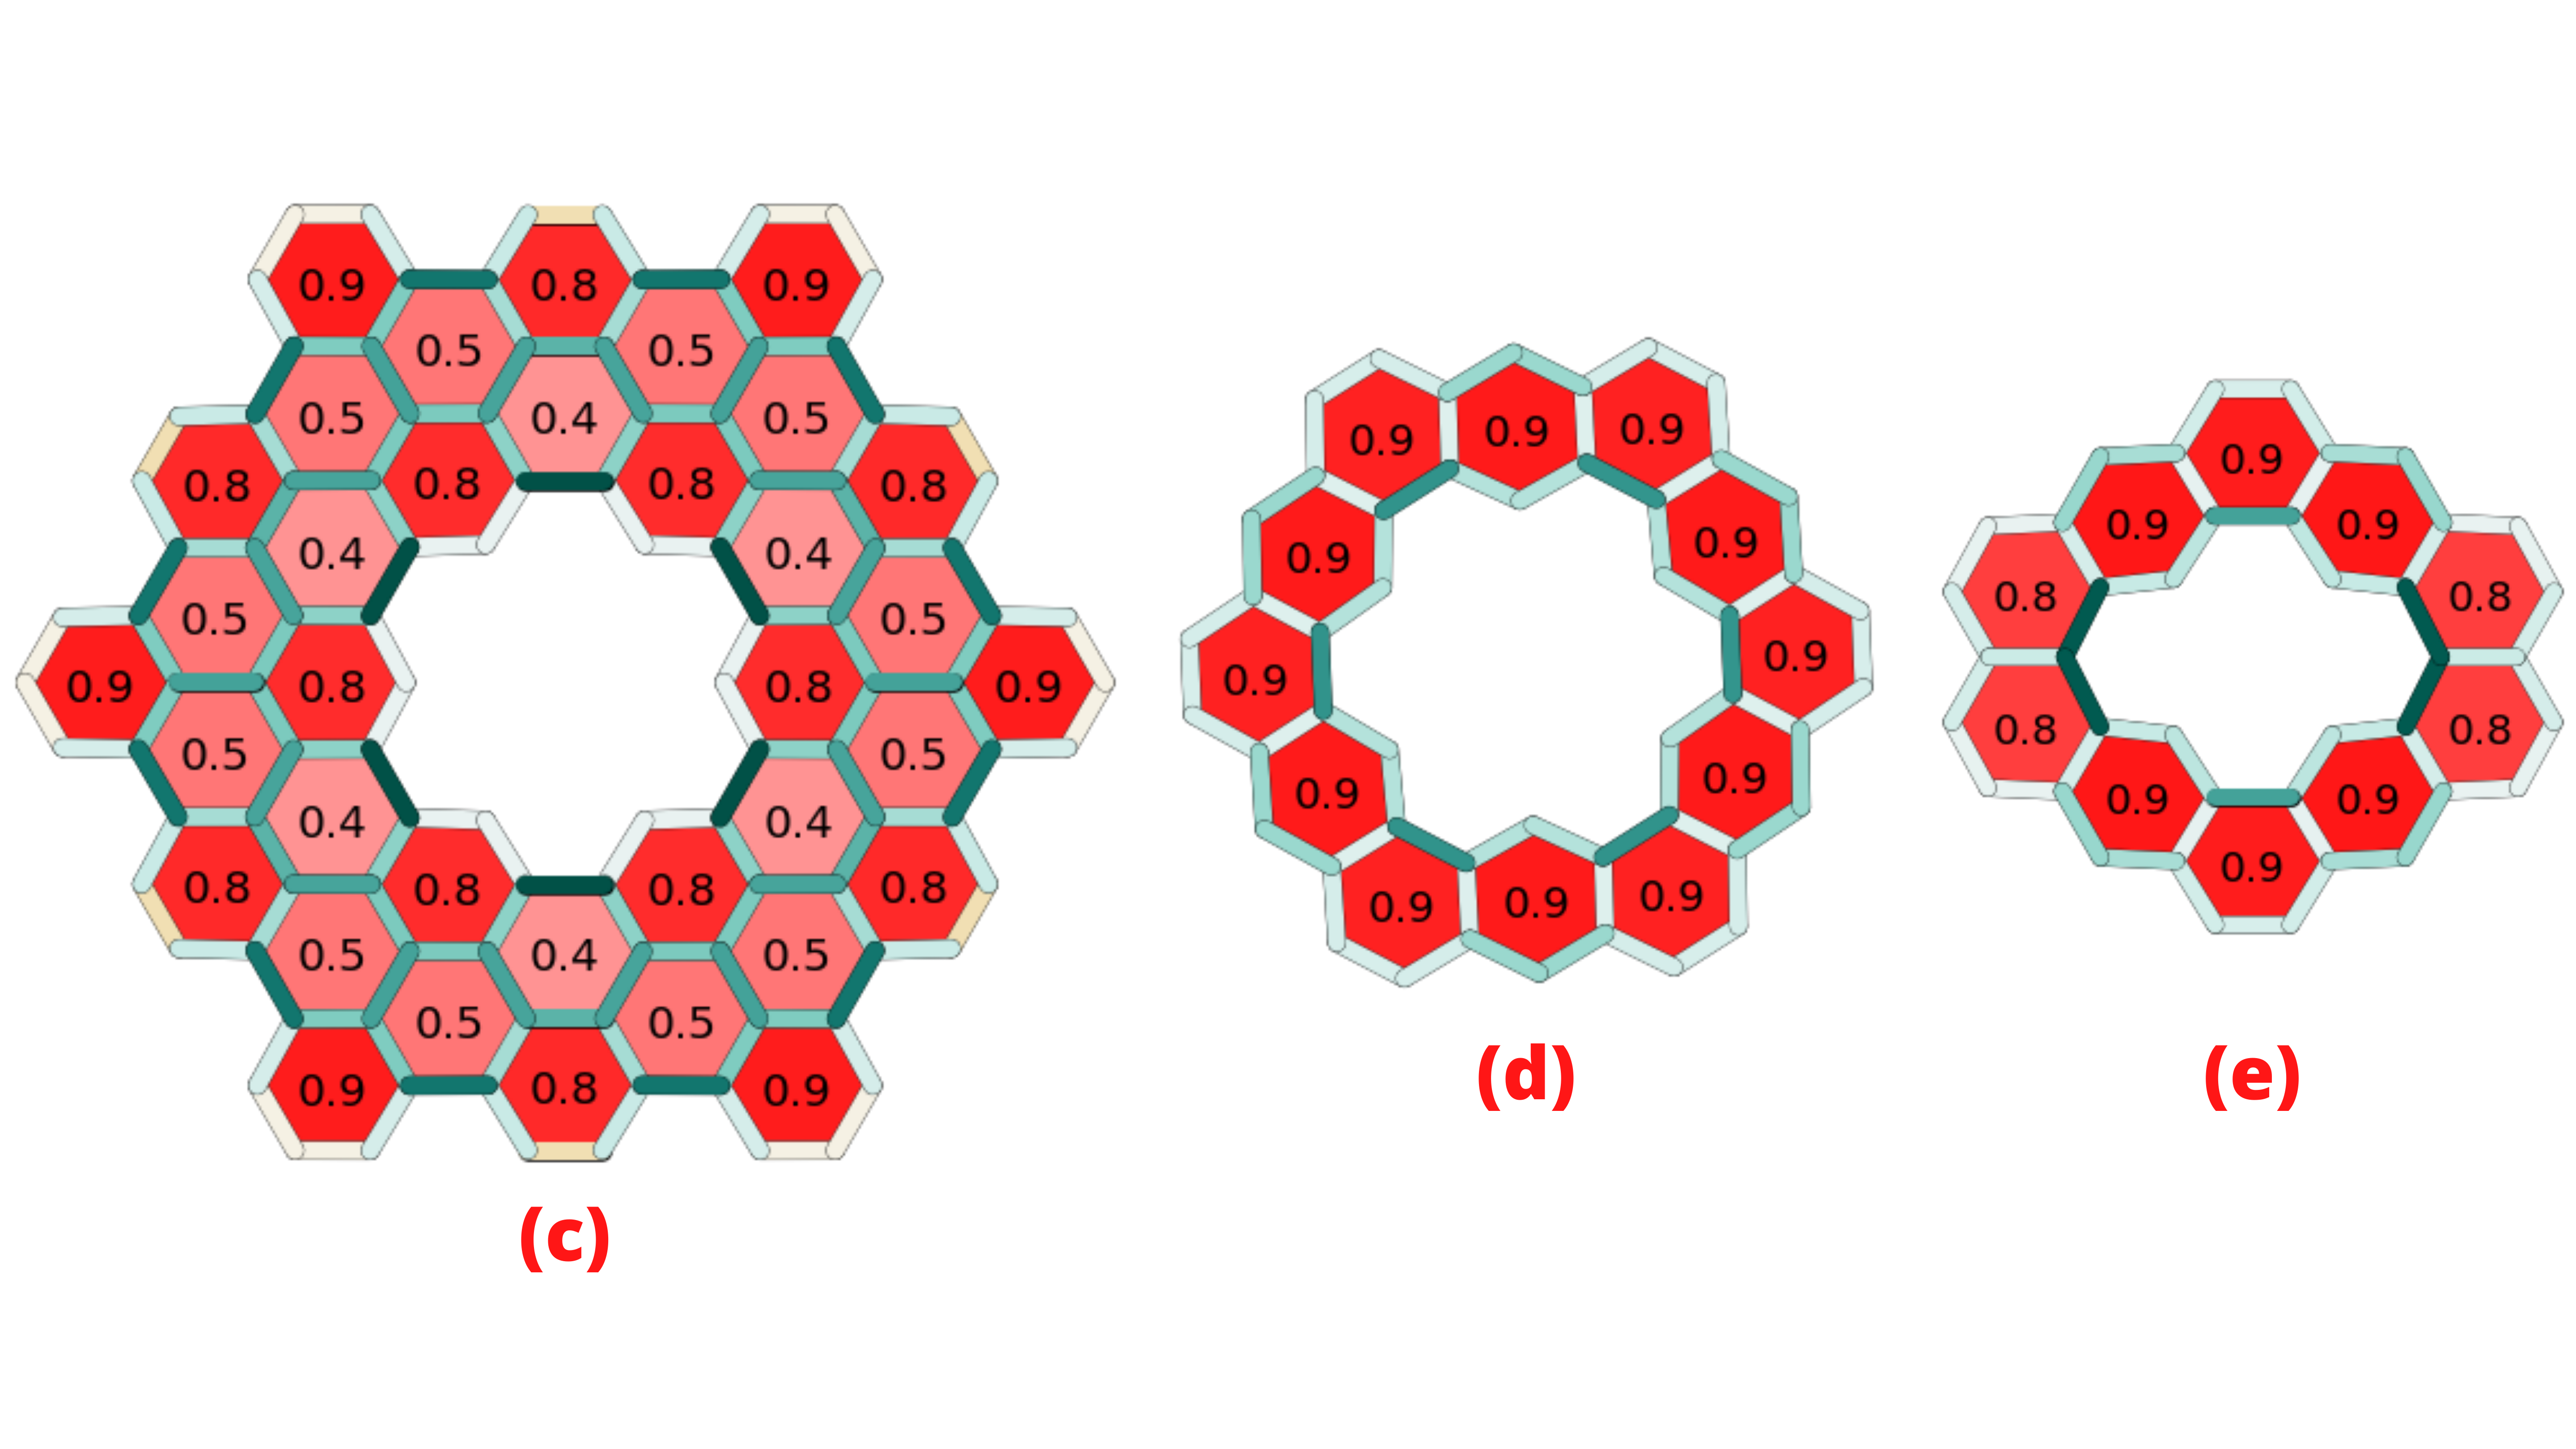
\includegraphics[width=1.0\textwidth]{images/15.png}
	\end{center}
	\fonte{Autor(a).}
\end{figure}

\subsection{Heterociclos aromáticos}

O efeito da ressonância em estruturas heterocíclicas depende da geometria do sistema e do tipo de heteroátomo presente no anel. No caso dos compostos que correspondem a anéis de cinco membros, como pirrol, furano, e seus derivados, são possíveis conjugações entre os pares de elétrons livres (do(s) heteroátomo(s)) e o sistema $\pi$. Consequentemente, são gerados híbridos de ressonância não equivalentes entre si, uma com separação de carga, e outra sem, não permitindo que a deslocalização eletrônica seja completa. Por outro lado, anéis de seis membros, a exemplo da piridina e seus derivados, apresentam conjugação $\pi-\pi$ total, com estruturas de ressonância que não têm separação de carga.

Após os efeitos de ressonância, os índices \gls{HOMED} (Tabela 11) calculados para as estruturas otimizadas do pirrol e do furano são inferiores aos dos heteroaromáticos de seis membros, como a piridina e o íon piranil, respectivamente. O índice \gls{HOMED} para o íon piranilíaco também é menor do que o índice para a piridina. Uma substituição do íon \ce{CH} pelo átomo N-aza em anéis com cinco membros parece reduzir o índice \gls{HOMED} em maior grau para O- que para N-derivados. Para anéis com seis membros, presença do átomo adicional N-aza em azinas não destrói o sistema de deslocalização completa de elétrons $\pi$ no sistema. Para os anéis de seis membros O-derivados, o índice \gls{HOMED} depende fortemente da posição do átomo N-aza. Ele diminui para posições 3 e 3,5; onde o átomo N pode estar próximo do átomo C+, e aumenta para a posição 4 onde o átomo N pode assumir a carga positiva.

\section{Análise estatística}

Para além dos resultados já mostrados, ainda é possível discutir o porquê do índice \gls{HOMA} ser a melhor alternativa para trabalhar com a aromaticidade a nível geométrico. Matematicamente, podemos interpretar o \gls{HOMA} como uma função matemática de objetos como o quadrado da distância em um espaço molecular abstrato de dimensão $n$. Chamemos ele de \gls{MS}, no qual uma molécula pode ser representada por um ponto $X = (x_1, x_2, \cdots, x_n)$, onde as coordenadas subsequentes correspondem aos comprimentos da ligação \ce{CC} selecionada. Uma comparação entre duas moléculas, $X$ e $Y$, pode ser expressa como uma distância $d(X, Y) = \displaystyle \sqrt{\sum_{i=1}^{n} (x_i - y_i)^2}$ no \gls{MS}. 

Essa comparação também faz sentido se estivermos interessados somente em uma diferença entre os fragmentos restritos, como os anéis, para avaliar sua aromaticidade. É suficiente dizer que, nessa definição:

\begin{equation}
    HOMA = 1 - \textit{const} \cdot d^2(X, Y)
\end{equation}

\noindent onde $d(\cdot)$ corresponde à distância no \gls{MS}, $X$ é um anel em uma dada molécula e $Y = (y_1, y_2, \cdots, y_n)$ é o benzeno, no qual todas as coordenadas são iguais entre si: $y_1 = y_2 = \cdots = y_n = y = d(CC)$. É uma representação espacial do que seria o $R_{opt}$ na \autoref{eq:3}. Por outro lado, \textit{const} corresponde ao fator $\alpha / n$ da \autoref{eq:3}. Adicionalmente, se nós assumirmos que existe uma molécula $Y$ na qual $y_1 = y_2 = \cdots = y_m = y = d(CC_{benzeno})$, mas $m \neq 6$, então nós calculamos o \gls{HOMA} para qualquer molécula composta por um número arbitrário de átomos de carbono.

No campo da estatística, o $k$-ésimo momento central da função de probabilidade de uma variável aleatória $x$, $\mu_k$, ou seja, o $k$-ésimo grau do valor esperado, é definido como se segue: $\mu_k = \langle (x - \langle x \rangle)^k \rangle = \displaystyle \frac{1}{n} \sum_{i = 1}^n (x_i - \bar{x})^k$, onde $\langle \bullet \rangle$ e $\bar{x}$ denotam a média aritmética.
Desse modo, o $k$-ésimo momento, $m_k = \langle x^k \rangle = \displaystyle \frac{1}{n} \sum_{i=1}^n (x_i)^k$, não é tomado sobre a média e $\mu_2 = m_2 - m_1^2$.

Então, se $x_i$ é identificado como o i-ésimo comprimento $R_i$ em uma molécula (um anel) e $\bar{x}$ como o $R_{opt}$, então o índice \gls{HOMA} está conectado à variância, que é o segundo momento central para as múltiplas variáveis discretas aleatórias: $x_1, x_2, \cdots, x_n$, ou seja, 

\begin{equation}
\label{statistic}
\begin{split}
    HOMA = 1 - \alpha \bigg[\frac{1}{n} \sum_{i=1}^n (x_i - \bar{x})^2 \bigg] = 1 - \alpha \cdot \mu_2 \\ = 1 - \alpha \cdot (m_2 - m_1^2 )
\end{split}
\end{equation}

\noindent onde o $\alpha$ corresponde à mesma constante de normalização da \autoref{eq:3}. Notemos que a \autoref{statistic} permite que $n$ seja maior do que 6 porque pode ser compreendido como o número de comparações com o comprimento de ligação ótimo. Ou seja, o índice \gls{HOMA} pode ser calculado para qualquer molécula composto por um número arbitrário de ligações \ce{CC}.

Uma vez que o índice \gls{HOMA} pode ser expresso como uma função linear de $d^2$ ou $\mu_2$, uma descrição melhor da aromaticidade geométrica pode ser buscada entre as extensões do \gls{HOMA}, o que é tratado como uma distância abstrata ou um parâmetro estatístico. Aqui, será explorada a abordagem estatística.

\begin{equation}
    \Gamma = 100 \cdot (\mu_1^\circ + \mu_2^\circ + \mu_3^\circ + \mu_4^\circ)
\end{equation}

\noindent onde $\mu_k = \displaystyle \frac{\mu_k}{(m_{1, ref})^k}$ e $m_{1, ref}$ é a média na molécula de referência. Dividindo $\mu_k$ pelo $k$-ésimo. Dividir $\mu_k$ pela potência de $m_{1, ref}$ garante a adimensionlidade do índice $\Gamma$.
% ---

% 5 - Conclusão
% ---
%\phantompart
\chapter{Conclusão}
% ----------------------------------------------------------

Por meio deste trabalho, foi apresentado o \textit{Balmy.jl}, uma aplicação \textit{web} capaz de auxiliar no cálculo de orbitais moleculares por meio do método de Hueckel estendido. Comprovou-se, através dos resultados, que as energias obtidas para os orbitais moleculares foram coerentes com a literatura original de Roald Hoffmann, criador da metodologia \gls{EHMO}. Os tempos de execução dos cálculos em comparação a um código já existente (\gls{YAeHMOP}) foram extremamente satisfatórios, com ganhos de 12.5\% em termos de desempenho e performance conforme aumentamos o número de bases no sistema. Isso ocorre devido às otimizações que a linguagem Julia possui para implementação de equações matemáticas em relação a outras linguagens, como C, por exemplo.

Os índices de quantificação da aromaticidade sob o ponto de vista geométrico também mostraram resultados que estão em bom acordo com a literatura. A abordagem estatística do índice de aromaticidade mostra como o \gls{HOMA} pode ser adotado enquanto o melhor descritor de aromaticidade geométrica, pois ele é baseado em uma fundamentação físico-química das energias e forças de ligação obtidas pela teoria do oscilador harmônico. Apesar disso, o índice \gls{HOMA} não é um bom descritor de aromaticidade para sistemas heteroaromáticos. Nesse sentido, o \textit{Balmy.jl} também contém o \gls{rHOMA} e o \gls{HOMED} implementados para análise de sistemas heterocíclicos aromáticos. De acordo com os resultados mostrados, o \gls{HOMED} é um melhor índice de heteroaromaticidade do que o \gls{rHOMA}, devido às parametrizações levando em conta sistemas aromáticos mínimos.
% ---

% ----------------------------------------------------------
% ELEMENTOS PÓS-TEXTUAIS
% ----------------------------------------------------------
\postextual
% ----------------------------------------------------------

% ----------------------------------------------------------
% Referências bibliográficas
% ----------------------------------------------------------
\begingroup
    \printbibliography[title=REFERÊNCIAS]
\endgroup

% ----------------------------------------------------------
% Glossário
% ----------------------------------------------------------
%
% Consulte o manual da classe abntex2 para orientações sobre o glossário.
%
%\glossary

% ----------------------------------------------------------
% Apêndices
% ----------------------------------------------------------

% ---
% Inicia os apêndices
% ---
\begin{apendicesenv}
%	\partapendices* 
	% ----------------------------------------------------------
\chapter{Descrição}
% ----------------------------------------------------------

Textos elaborados pelo autor, a fim de completar a sua argumentação. Deve ser precedido da palavra APÊNDICE, identificada por letras maiúsculas consecutivas, travessão e pelo respectivo título. Utilizam-se letras maiúsculas dobradas quando esgotadas as letras do alfabeto. 

\begin{quadro}[htb]
	\centering
	\caption{\label{qua:Quadro_2}Modelo A.}	
\begin{tabular}{|l|l|}
\hline
xxxx              & yyyyyyyyyyyyyyy    \\
\hline
xxxx              & yyyyyyyyyyyyyyy    \\
\hline
xxxx              & yyyyyyyyyyyyyyy    \\
\hline
xxxx              & yyyyyyyyyyyyyyy    \\
\hline
xxxx              & yyyyyyyyyyyyyyy    \\
\hline
xxxx              & yyyyyyyyyyyyyyy    \\
\hline
xxxx              & yyyyyyyyyyyyyyy    \\
\hline
rrrrrrrrrrrrrrrrr & eeeeeeeeeeeeeeeee  \\
\hline
xxxx              & yyyyyyyyyyyyyyy    \\
\hline
xxxx              & yyyyyyyyyyyyyyy    \\
\hline
rrrrrrrrrrrrrrrrr & eeeeeeeeeeeeeeeee  \\
\hline
xxxx              & yyyyyyyyyyyyyyy    \\
\hline
                  & ttttttttttttttttt  \\
\hline
rrrrrrrrrrrrrrrrr & eeeeeeeeeeeeeeeee  \\
\hline
ttttttttttttt     &                    \\
\hline
rrrrrrrrrrrrrrrrr & eeeeeeeeeeeeeeeee  \\
\hline
rrrrrrrrrrrrrrrrr & eeeeeeeeeeeeeeeee  \\
\hline
                  & gggggggggggggggggg \\
\hline
rrrrrrrrrrrrrrrrr & eeeeeeeeeeeeeeeee  \\
\hline
rrrrrrrrrrrrrrrrr & eeeeeeeeeeeeeeeee  \\
\hline
rrrrrrrrrrrrrrrrr & eeeeeeeeeeeeeeeee  \\
\hline
rrrrrrrrrrrrrrrrr & eeeeeeeeeeeeeeeee  \\
\hline
\end{tabular}
\fonte{Elaborada pelo autor (2016).}
\end{quadro}
\end{apendicesenv}
% ---


% ----------------------------------------------------------
% Anexos
% ----------------------------------------------------------

% ---
% Inicia os anexos
% ---
\begin{anexosenv}
%	\partanexos*
	% ----------------------------------------------------------
\chapter{Descrição}
% ----------------------------------------------------------

São documentos não elaborados pelo autor que servem como fundamentação (mapas, leis, estatutos). Deve ser precedido da palavra ANEXO, identificada por letras maiúsculas consecutivas, travessão e pelo respectivo título. Utilizam-se letras maiúsculas dobradas quando esgotadas as letras do alfabeto. 

\end{anexosenv}

%---------------------------------------------------------------------
% INDICE REMISSIVO
%---------------------------------------------------------------------
%\phantompart
%\printindex
%---------------------------------------------------------------------

\end{document}
